% Created 2022-01-10 ma 11:21
% Intended LaTeX compiler: pdflatex
\documentclass[12pt]{article}

%%%% settings when exporting code %%%% 

\usepackage{listings}
\lstdefinestyle{code-small}{
backgroundcolor=\color{white}, % background color for the code block
basicstyle=\ttfamily\small, % font used to display the code
commentstyle=\color[rgb]{0.5,0,0.5}, % color used to display comments in the code
keywordstyle=\color{black}, % color used to highlight certain words in the code
numberstyle=\ttfamily\tiny\color{gray}, % color used to display the line numbers
rulecolor=\color{black}, % color of the frame
stringstyle=\color[rgb]{0,.5,0},  % color used to display strings in the code
breakatwhitespace=false, % sets if automatic breaks should only happen at whitespace
breaklines=true, % sets automatic line breaking
columns=fullflexible,
frame=single, % adds a frame around the code (non,leftline,topline,bottomline,lines,single,shadowbox)
keepspaces=true, % % keeps spaces in text, useful for keeping indentation of code
literate={~}{$\sim$}{1}, % symbol properly display via latex
numbers=none, % where to put the line-numbers; possible values are (none, left, right)
numbersep=10pt, % how far the line-numbers are from the code
showspaces=false,
showstringspaces=false,
stepnumber=1, % the step between two line-numbers. If it's 1, each line will be numbered
tabsize=1,
xleftmargin=0cm,
emph={anova,apply,class,coef,colnames,colNames,colSums,dim,dcast,for,ggplot,head,if,ifelse,is.na,lapply,list.files,library,logLik,melt,plot,require,rowSums,sapply,setcolorder,setkey,str,summary,tapply},
aboveskip = \medskipamount, % define the space above displayed listings.
belowskip = \medskipamount, % define the space above displayed listings.
lineskip = 0pt} % specifies additional space between lines in listings
\lstset{style=code-small}
%%%% packages %%%%%

\usepackage[utf8]{inputenc}
\usepackage[T1]{fontenc}
\usepackage{lmodern}
\usepackage{textcomp}
\usepackage{color}
\usepackage{graphicx}
\usepackage{grffile}
\usepackage{wrapfig}
\usepackage{rotating}
\usepackage{longtable}
\usepackage{multirow}
\usepackage{multicol}
\usepackage{changes}
\usepackage{pdflscape}
\usepackage{geometry}
\usepackage[normalem]{ulem}
\usepackage{amssymb}
\usepackage{amsmath}
\usepackage{amsfonts}
\usepackage{dsfont}
\usepackage{array}
\usepackage{ifthen}
\usepackage{hyperref}
\usepackage{natbib}
%
%%%% specifications %%%%
%
\usepackage{ifthen}
\usepackage{xifthen}
\usepackage{xargs}
\usepackage{xspace}
\newcommand\Rlogo{\textbf{\textsf{R}}\xspace} %
\RequirePackage{fancyvrb}
\DefineVerbatimEnvironment{verbatim}{Verbatim}{fontsize=\small,formatcom = {\color[rgb]{0.5,0,0}}}
\usepackage{titlesec} % rename appendix
\usepackage{etoolbox}
\makeatletter
\patchcmd{\ttlh@hang}{\parindent\z@}{\parindent\z@\leavevmode}{}{}
\patchcmd{\ttlh@hang}{\noindent}{}{}{}
\makeatother
\RequirePackage{colortbl} % arrayrulecolor to mix colors
\RequirePackage{setspace} % to modify the space between lines - incompatible with footnote in beamer
\renewcommand{\baselinestretch}{1.1}
\geometry{top=1cm,bottom=2cm}
\usepackage{changepage}
\hypersetup{
citecolor=[rgb]{0,0.5,0},
urlcolor=[rgb]{0,0,0.5},
linkcolor=[rgb]{0,0,0.5},
}
\RequirePackage{epstopdf} % to be able to convert .eps to .pdf image files
\RequirePackage{capt-of} %
\RequirePackage{caption} % newlines in graphics
\usepackage{placeins}
\author{Brice Ozenne, \today}
\date{}
\title{CAR project: computation of the AUC based on 3 sampling points}
\hypersetup{
 colorlinks=true,
 pdfauthor={Brice Ozenne, \today},
 pdftitle={CAR project: computation of the AUC based on 3 sampling points},
 pdfkeywords={},
 pdfsubject={},
 pdfcreator={Emacs 27.2 (Org mode 9.4.4)},
 pdflang={English}
 }
\begin{document}

\maketitle

\section{Background}
\label{sec:org6b65cbe}

Cortisol awakening response (CAR) describes the period of sharp
increase in cortisol secretion in the first 60 min after awakening. It
is used in various clinical studies, including studies on the
serotonin transporter or on serotonin 4 receptors.

\bigskip

CAR is usually estimated using saliva samples obtained immediately
upon awakening, and at 15, 30, 45, and 60 minutes after
awakening. First, the concentration in cortisol in each saliva sample
is measured. The five measurements are then used to represent the
temporal evolution of the cortisol concentration (see
\autoref{fig:trajLCMM-homo}).

\bigskip

The CAR curve is then summarized either into the area under the curve
with respect to increase (\(AUC_I\)) or the area under the curve
(\(AUC_G\)). \(AUC_G\) corresponds to the average concentration value
multiplied by the duration of the experiment (here 60 minutes) while
\(AUC_I\), as defined by \cite{fekedulegn2007area}, can be computed as
\(AUC_I = AUC_G - AUC_B\) where \(AUC_B\) is the baseline cortisol
value times the follow-up time (here 60 min). We note that since
\(AUC_B\) is estimated in the same way with 3 or 5 samples, the
properties of \(AUC_I\) can be deduced from the one of \(AUC_G\). This
is why we will focus on the estimation of \(AUC_G\) in the aim and
method sections. Nevertheless we will report results for the
estimation of the \(AUC_I\).


\begin{figure}[!h]
\centering
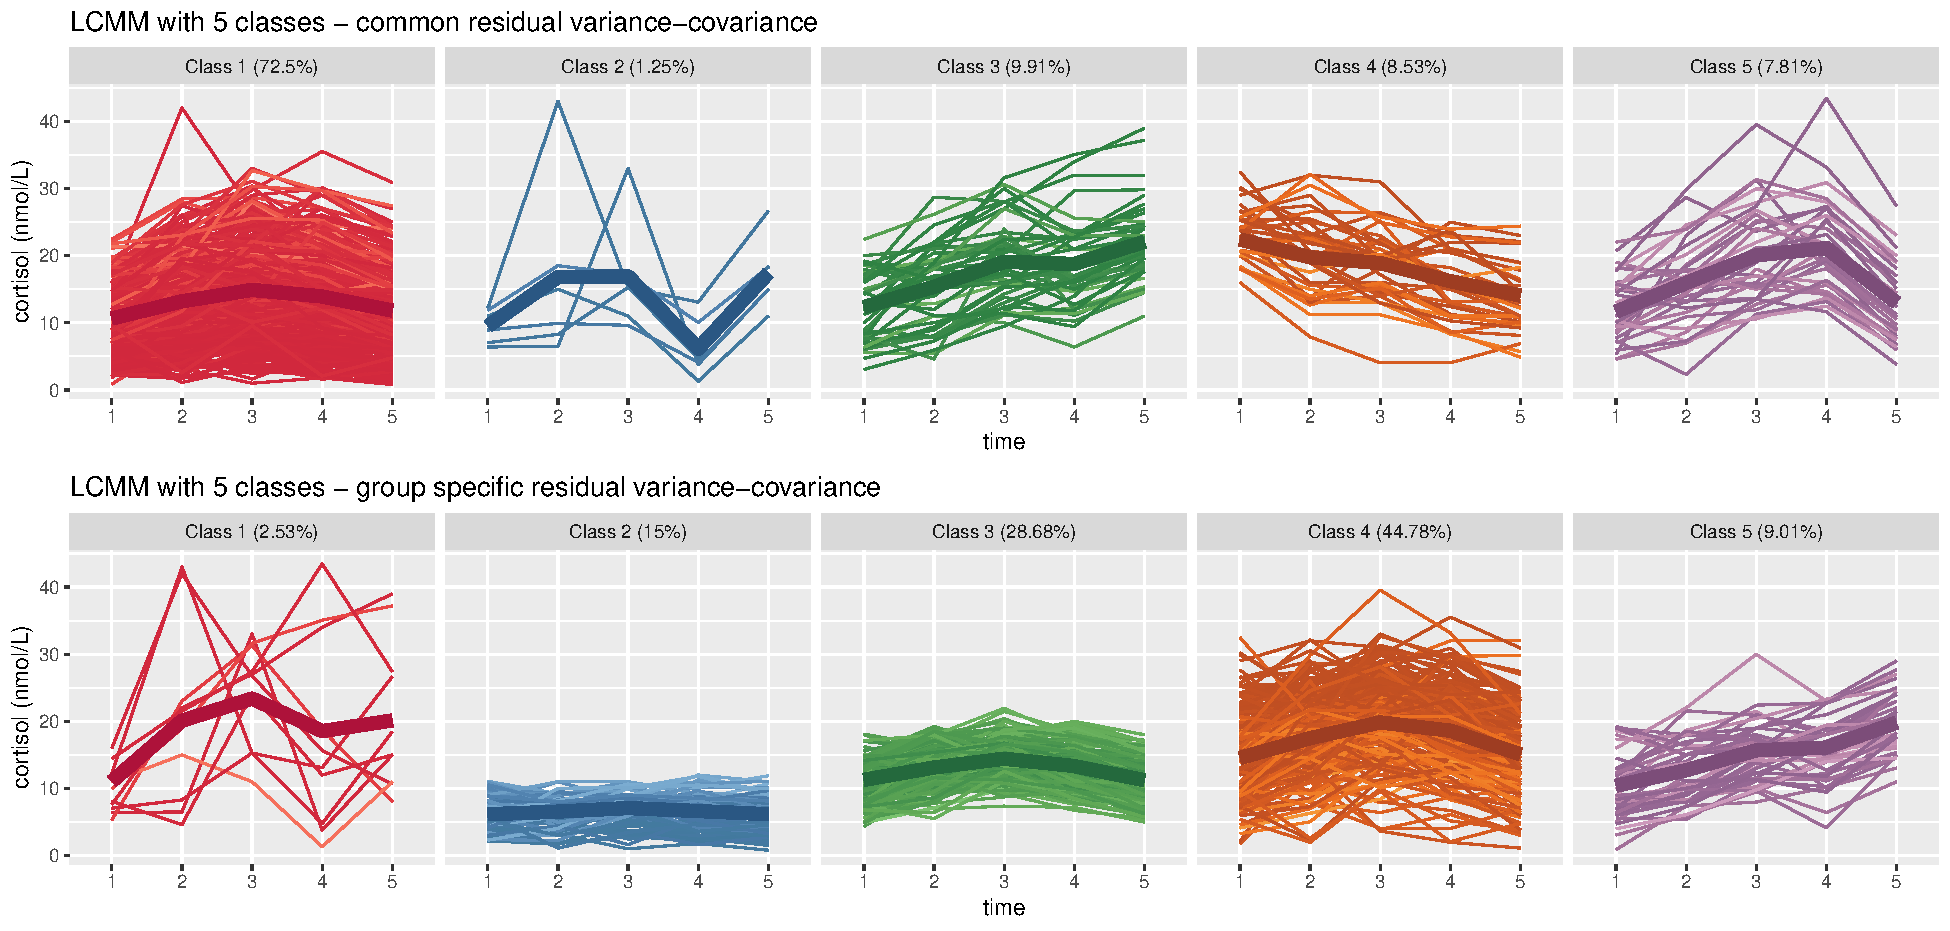
\includegraphics[width=\textwidth]{./figures/trajLCMM-5groups.pdf}
\caption{\label{fig:trajLCMM-homo}Trajectories of the cortisol concentration over time in healthy individuals with 5 measurement and a \(AUC_G\) below 2000. Trajectories were divided into 5 classes according to two different latent class linear mixed models (row 1 and row 2). The brightness of the color reflects the membership probability to the class.}
\end{figure}

\FloatBarrier

\section{Aim}
\label{sec:org2d36cb4}

The project's aim is to assess the reliability of an estimator of the
CAR based on only 3-samples (instead of the usual 5). Three aspects
should be discussed:
\begin{itemize}
\item \textbf{Parameter of interest}: the parameter of interest are the
\(AUC_I\) and \(AUC_G\) which seems also to be commonly used in the
litterature. \newline \emph{However} their value depends on the duration
of the cortisol measurements which can be problematic:
\begin{description}
\item[{(i)}] when subjects do not followed the scheduled measurement
times, e.g. subject 10834 has samples at time 9h16, 9h30,
9h45, 10h00, 10h15, i.e. was 1 minute too early at his
second measurement so his \(AUC_G\) which will be biased
toward 0 compared to what we would have computed has the
subject followed the schedule.
\item[{(ii)}] when changing the sampling strategy, e.g.  only using
measurements up to 30 min (instead of 60 min) will lead
to a systematically lower \(AUC_G\).
\end{description}
 A "good" parameter of interest should be independent of the study
design (i.e. sampling strategy). A possible remedie would be to
consider the \(AUC_I\) or \(AUC_G\) \emph{per hour}.

\item \textbf{Estimators of the \(AUC_G\)}: currently the method used to
estimate the \(AUC_G\) is the \emph{trapezoidal rule}, i.e., using a
weighted sum of the cortisol measurements where the weights are a
function of the measurement times (see appendix \ref{appendix:trapezRule} for
an example). \newline One could also try a more \emph{data driven
method}, i.e. learn on a dataset what are the optimal weights to
match the 5-samples AUC value. This approach is especially relevant
for correcting the shorter observation time: we can for instance
weight more each measurement when using only the 0, 15, and 30
minute samples and get a 3-sample estimator of the \(AUC_G\) that is
no more downward biased \footnote{More complex learning strategies could be used to better handle
various types of trajectories. For instance, if the cortisol
concentration is always decreasing over time, weighting more each
measurement will not be a valid solution when using only the 0, 15,
and 30 minutes samples. But to keep things simple, we will not look
into that.}.

\item \textbf{Assessment}: Ideally we would like to assess both the
accuracy and the precision of our new estimators of the
\(AUC_G\). For instance, consider indivividuals with the same CAR
but different trajectories, we would like to know whether in average
we estimate the right value (accuracy) and how by how much our
estimates fluctuates over individuals (precision). To do so we
should compare our estimates to the true value and thus obtain
residuals. The accuracy can quantified based on the mean (or median)
of the residuals and the precision based on the variance (or
quantiles) of the residuals. Sometime we don't require to estimate
the right value, but only that up to a (possibly unknwon)
transformation, we estimate the right value \footnote{e.g. the correlation/covariance between \(AUC_G\) and PET values
would be insensitive to linear transformations of the \(AUC_G\).}. In that case,
correlation coefficients can be of interest. We will report the
Pearson's correlation coefficient which corresponds to a linear
transformation. \newline \emph{Unfortunately} we don't have access to a
"truth" for the \(AUC_G\) values. Instead we will use the \(AUC_G\)
estimated using 5-measurements as a proxy for the "truth".
\end{itemize}

\section{Method}
\label{sec:org9bbdfc4}

\subsection{Training data}
\label{sec:orgceb6c8e}

The full dataset contains 984 series of cortisol measurements both
from healthy individuals and patients. The following exclusion
criteria were applied:
\begin{description}
\item[{(i)}] wake-up time posterior to the time of first sample or time of
first sample later than 15 minutes after wake-up time (16 individuals).
\item[{(ii)}] time of first sample posterior to the time of second sample
or time of second sample later than 20 minutes after time of
first sample (8 individuals). Same for third (20
individuals), fourth (23 individuals), and fifth (23
individuals) sample.
\item[{(iii)}] at least one missing cortisol measurement (86 individuals)
\item[{(iv)}] at least one missing measurement time (21 individuals)
\end{description}
Note that the same individual may appear in several exclusion
  criteria; see appendix \ref{appendix:exclusion} for details. In total, it
  remains 815 trajectories belonging to 540 distinct individuals, 470
  trajectores originating from 325 healthy individuals and 345
  trajectories originating from 215 patients. In what follows we will
  not take into account that some series originates from the same
  patient and call a serie of 5 cortisol measurements a trajectory.

\bigskip

The calculation of the \(AUC_G\) was performed based on the
trapezoidal rule (R function \texttt{pracma::trapz}) and matched the
\(AUC_G\) values present in the datatest. There was also very close
aggreement between the \(AUC_I\) computed in R and from the
database. However there were significant discripancy in \(AUC_B\) (see
appendix \ref{appendix:trapezRule} for detail) but since they are not used
later on this is not considered an issue.

\bigskip

For the exploratory analysis and for training the statistical models,
we will only consider the healthy controls with no missing values
(i.e. all 5 samples). As shown in \autoref{fig:alltraj-HC} there are
some clear outliers. To simplify visualization and modeling, they were
excluded by removing all trajectories having a \(AUC_g\)
above 2000. When using the cases as testing set, individuals with
large \(AUC_g\) were also excluded (here \(AUC_g>5000\)). In both the
training and test set individuals with delayed measurements (first
sample more than 15 min after wake up, or more than 5 minutes delay in
following measurements) were also excluded.

\begin{figure}[!h]
\centering
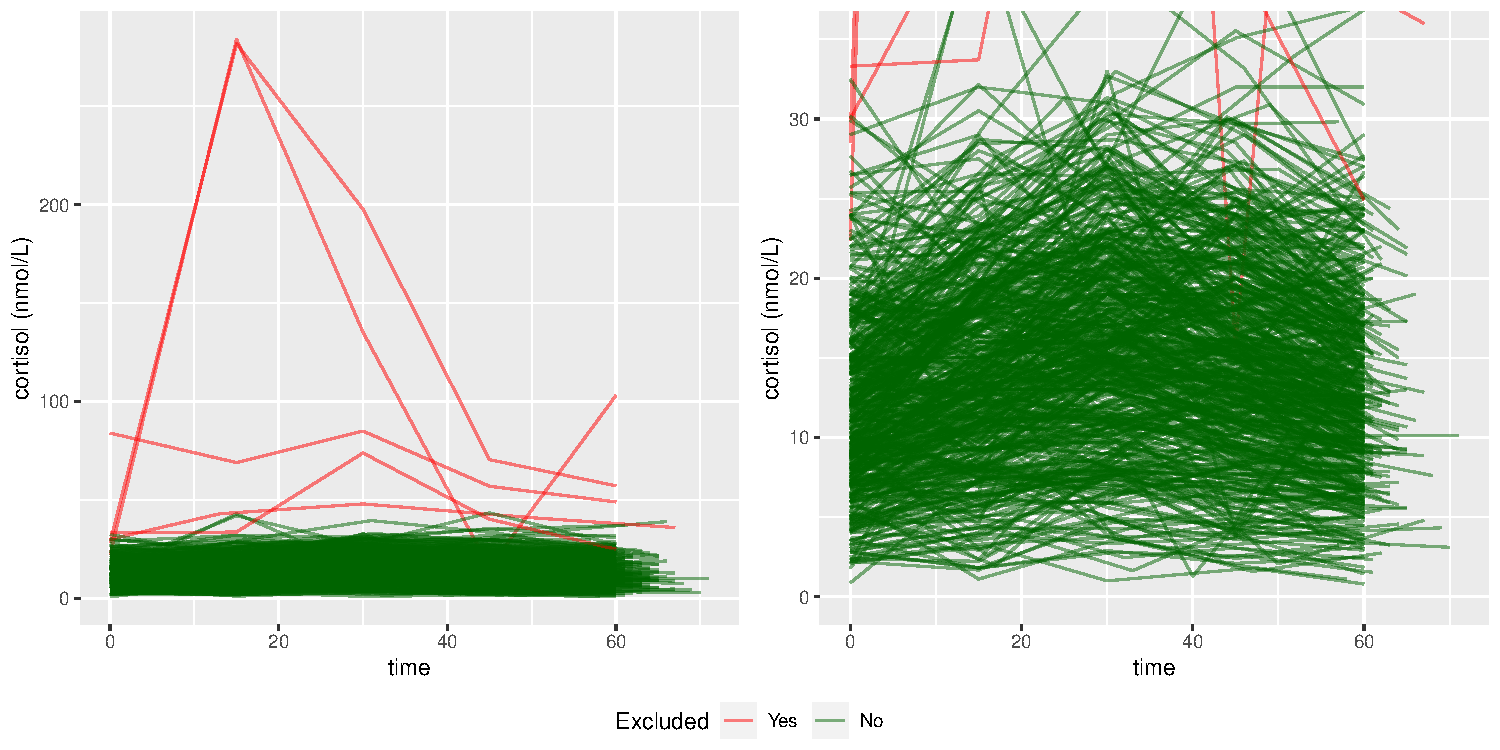
\includegraphics[width=\textwidth]{./figures/cortisol-individual-alltraj.pdf}
\caption{\label{fig:alltraj-HC}Individual cortisol trajectories in the healthy controls. The colors indicate whether a trajectory was used in the exploratory analysis and training of the statistical model.}
\end{figure} 

\subsection{Statistical analysis}
\label{sec:org40670d8}

\textbf{Exploratory}: Identifing typical shapes of trajectories can help to
decide which three samples to use. For instance if two trajectories
start the same but differ at latter timepoints, it may not be possible
to get an accurate AUC based only on the first measurements
(e.g. consider class 2 and 3 in row 1 of
\autoref{fig:trajLCMM-homo}). Latent class linear mixed models (LCMM)
were used to try to identify these typical trajectories and estimate
the percentage of observations associated to each typical trajectory.
The number of classes (i.e. typical trajectories) was varied from 1
to 6. A different mean parameter was estimated for each class and
timepoint. An unstructured covariance matrix was used to model the
covariance between the residuals (within trajectory). Two types of
LCMM were fitted: one where the covariance matrix is assumed to be the
same for all classes and another where it is class specific. \newline
\textcolor{red}{WARNING}: to save computation time each
model was run using a single initialization. One would need to compare
several initializations to check the stability of the results.

\bigskip

\textbf{Evaluation of the estimators}: The \(AUC_G\) for with 5-samples was
computed using the trapezoidal rule and used as a gold standard. The
3-samples \(AUC_G\) was computed either using the trapezoidal rule or
using the linear predictor of a linear regression. The linear
regression was fitted using the 5-sample \(AUC_G\) as an outcome, the
\(AUC_G\) estimated by the trapezoidal rule on 3-samples as an offset,
and the 3 cortisol values multiplied by the time intervals as
regressors (see appendix \ref{appendix:lm} for details). We always used the
first sample (0 minute) and two of the four following samples (15, 30,
45, or 60 minutes). This gives rise to 2*6 estimators.\newline These
estimators were evaluted on the healthy control dataset (when using
the linear regression, a 10-fold cross validation was used) and on the
patient dataset. \newline Note that, because \(AUC_B\) does not vary
over estimators, the estimation error for the \(AUC_I\) will be the
same as for the \(AUC_G\). The correlation between the 3 and 5-sample
estimators may differ though. We won't report relative error because
it is not well defined as it requires to divide by \(AUC_I\) (which
may be null).

\section{Results}
\label{sec:org75128ed}

\subsection{Exploratory analysis}
\label{sec:org9de8ae1}

As shown in \autoref{tab:lcmm}, all LCMM but one converged (common
variance, 6 classes). Visual inspection of the class trajectories
suggested to retain the 5 class model \footnote{this is a bit arbitrary.}.
\autoref{fig:trajLCMM-homo} shows the typical trajectories estimated for
each class along with the observed trajectories belonging to that
class. Some patterns were identified:
\begin{itemize}
\item \emph{inverse V shape trajectory}: increase then decrease. About about 8\%
of the trajectories according the LCMM with common variance
(row 1 Class 5).
\item \emph{monotone trajectory}: increase or decrease. About 9\% of the
trajectories (row 1 Class 3 and 4 and row 2 class 5).
\item \emph{stable trajectory}. About 15\% of the trajectories were rather
constant, fluctuating only between rather low values (row 2 Class
2).
\item \emph{very variable trajectory}. A few percents (row 1 Class 2 and row 2
Class 1).
\end{itemize}
Unfortunately for still a rather large proportion of trajectories
(70\%, row 1 Class 1 or row 2 Class 3 and 4), no clear pattern was
identified. This show the limits of this "generic" LCMM
approach. Better shape identification might be possible with an model
specifically design for this problem (but this would require much more
work!). For the previous types, one would expect that using 3-samples
at time 0, 30, and 60 to give a reasonnable approximation - with the
exception of the few \emph{very variable trajectory}. Considering only
early (0, 15, and 30 minutes) or only late (30, 45, and 60 minutes) is
unlikely to be satisfying since one would not be able to distinguish
between monotonic and inverse V shape trajectories. This is
problematic since these represent a non-neglectable proportion of the
sample.

\subsection{Evaluation of the estimators: 3 vs. 5-sample \(AUC_G\)}
\label{sec:org8156e7b}

From the estimated coefficients of the linear regression
(\autoref{tab:coeflm}), it appears that the trapezoidal rule tends to
underestimate the \(AUC_G\) (positive intercept in all models). In
models not including the 60 minute sample, the last sample was given
additional weight compared to the trapezoidal rule to further correct
the downward bias. The weights of the other samples were essentially
unchanged.

\bigskip

The performance of the estimators are displayed in
\autoref{fig:AUCg-perf-estimator} and summarized in
\autoref{tab:AUCg-perfEstimator}. Performance between the training
(i.e. healthy controls) and test set (i.e. patients) were very
similar.  While all estimators showed high correlation with the
5-sample \(AUC_G\) (see \autoref{fig:AUCg-cor-estimator} for a visual
representation of the impact of the estimator on the correlation),
they greatly differ in term of accuracy and precision.

\bigskip

When using the trapezoidal rule, as expected, all estimators not
including the 60 minute sample were downward biased. Moreover the
0-15-30 was vary variable. Overall using the samples 0, 30 minutes,
and 60 minutes lead to the least bias (about -10 nmol.h/L or -1\%) and
least variation (about 65 nmol.h/L or 8\%). The other estimators
showed much higher bias and/or variability and are not recommanded.

\bigskip

The linear regression had very little impact on the 0-15-30 estimator
(as shown in \autoref{tab:coeflm}). For all other estimators, it
corrected most of the bias and greatly reduced their variability. With
this approach the 0-15-45 and 0-30-45 estimators become an option with
a bias of about +/- 5 nmol.h/L (0.5\%) and fluactuation of about 60
nmol.h/L (7\%). \autoref{fig:AUCg-cor-estimator} can also be used to see
the accuracy and precision along the \(AUC_G\) value. They don't seem
to vary much for the recommanded estimators - compare to the estimator
trapezoidal rule 0-15-30 whose precision decreases (i.e. the variance
increases) when looking at higher \(AUC_G\) values. This may be easier
to see when considering the relative error along the AUCg values
(\autoref{fig:AUCg-bland-estimator}).

\begin{figure}[!h]
\centering
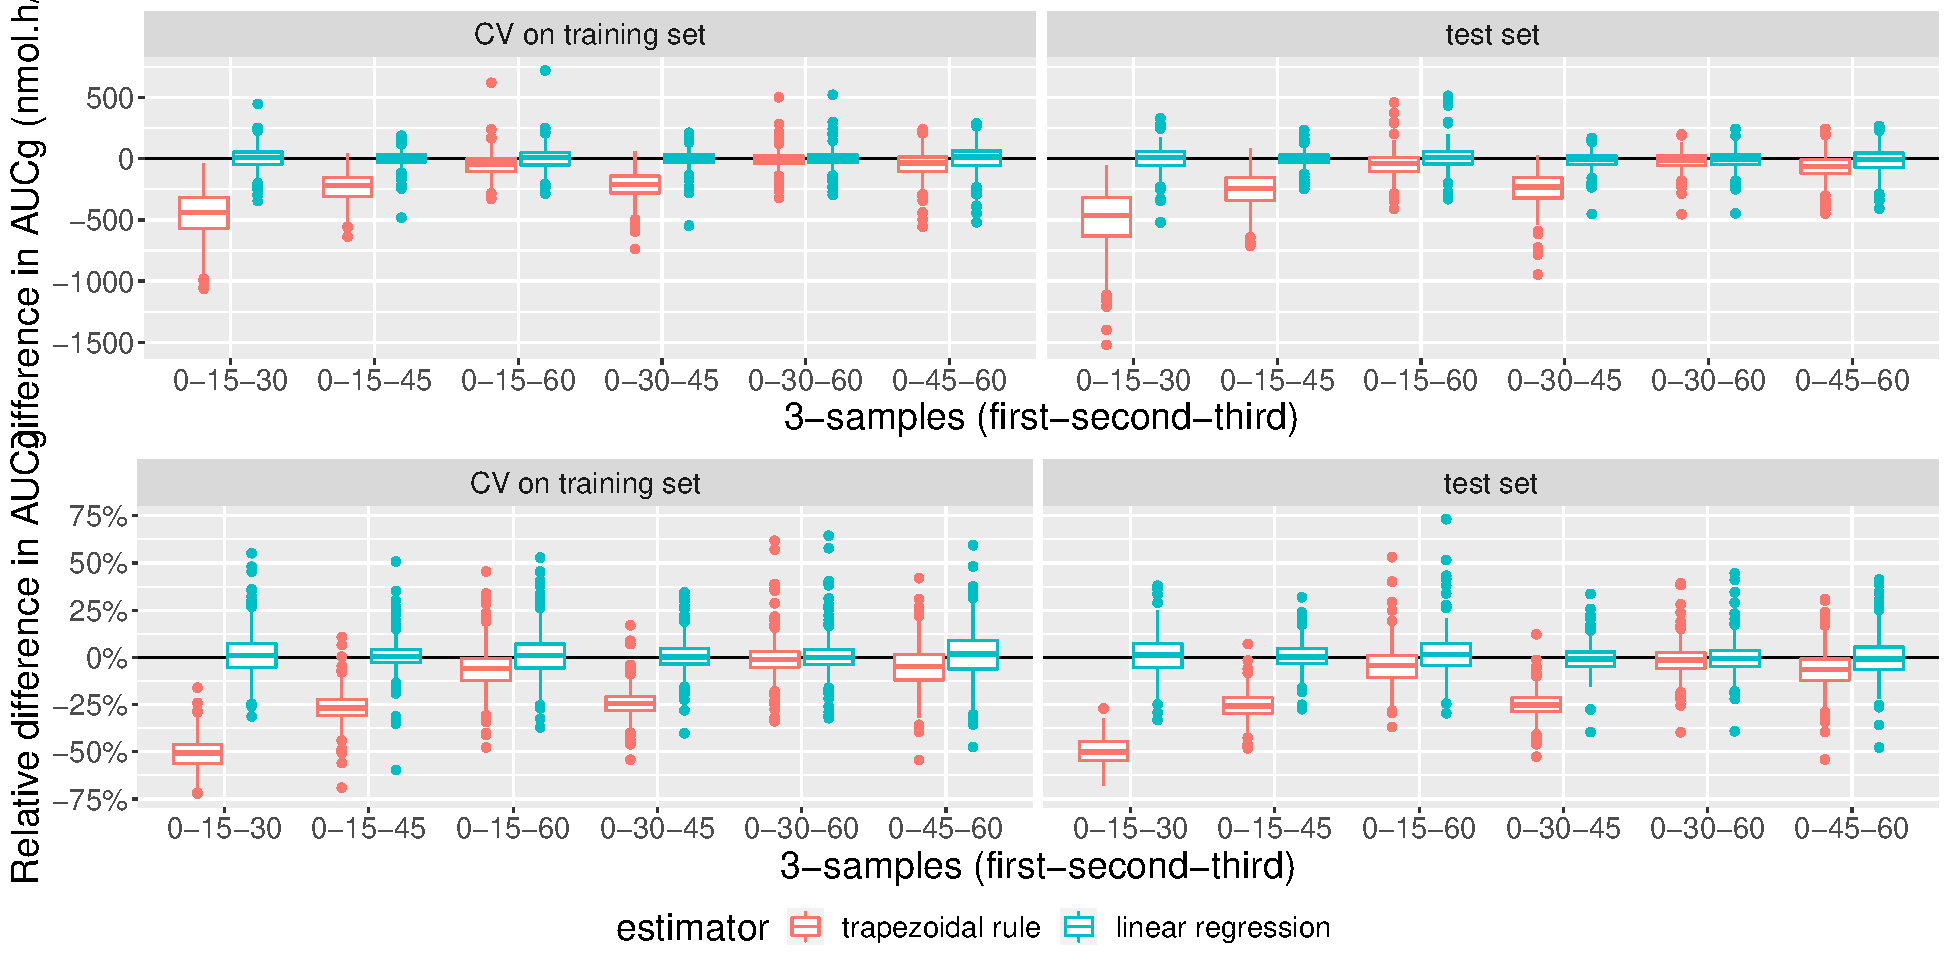
\includegraphics[width=1\textwidth]{./figures/AUCg-perf-boxplot.pdf}
\caption{\label{fig:AUCg-perf-estimator}Boxplot of the difference between the estimated 5-sample \(AUC_G\) and the estimated 3-sample \(AUC_G\). The closer to 0 the better. The first row displays the difference in unit of cortisol concentration (summed over an hour) while the second row display the relative difference (unitless), i.e. the difference divided by the estimated 5-sample \(AUC_G\).}
\end{figure}

\begin{figure}[!h]
\centering
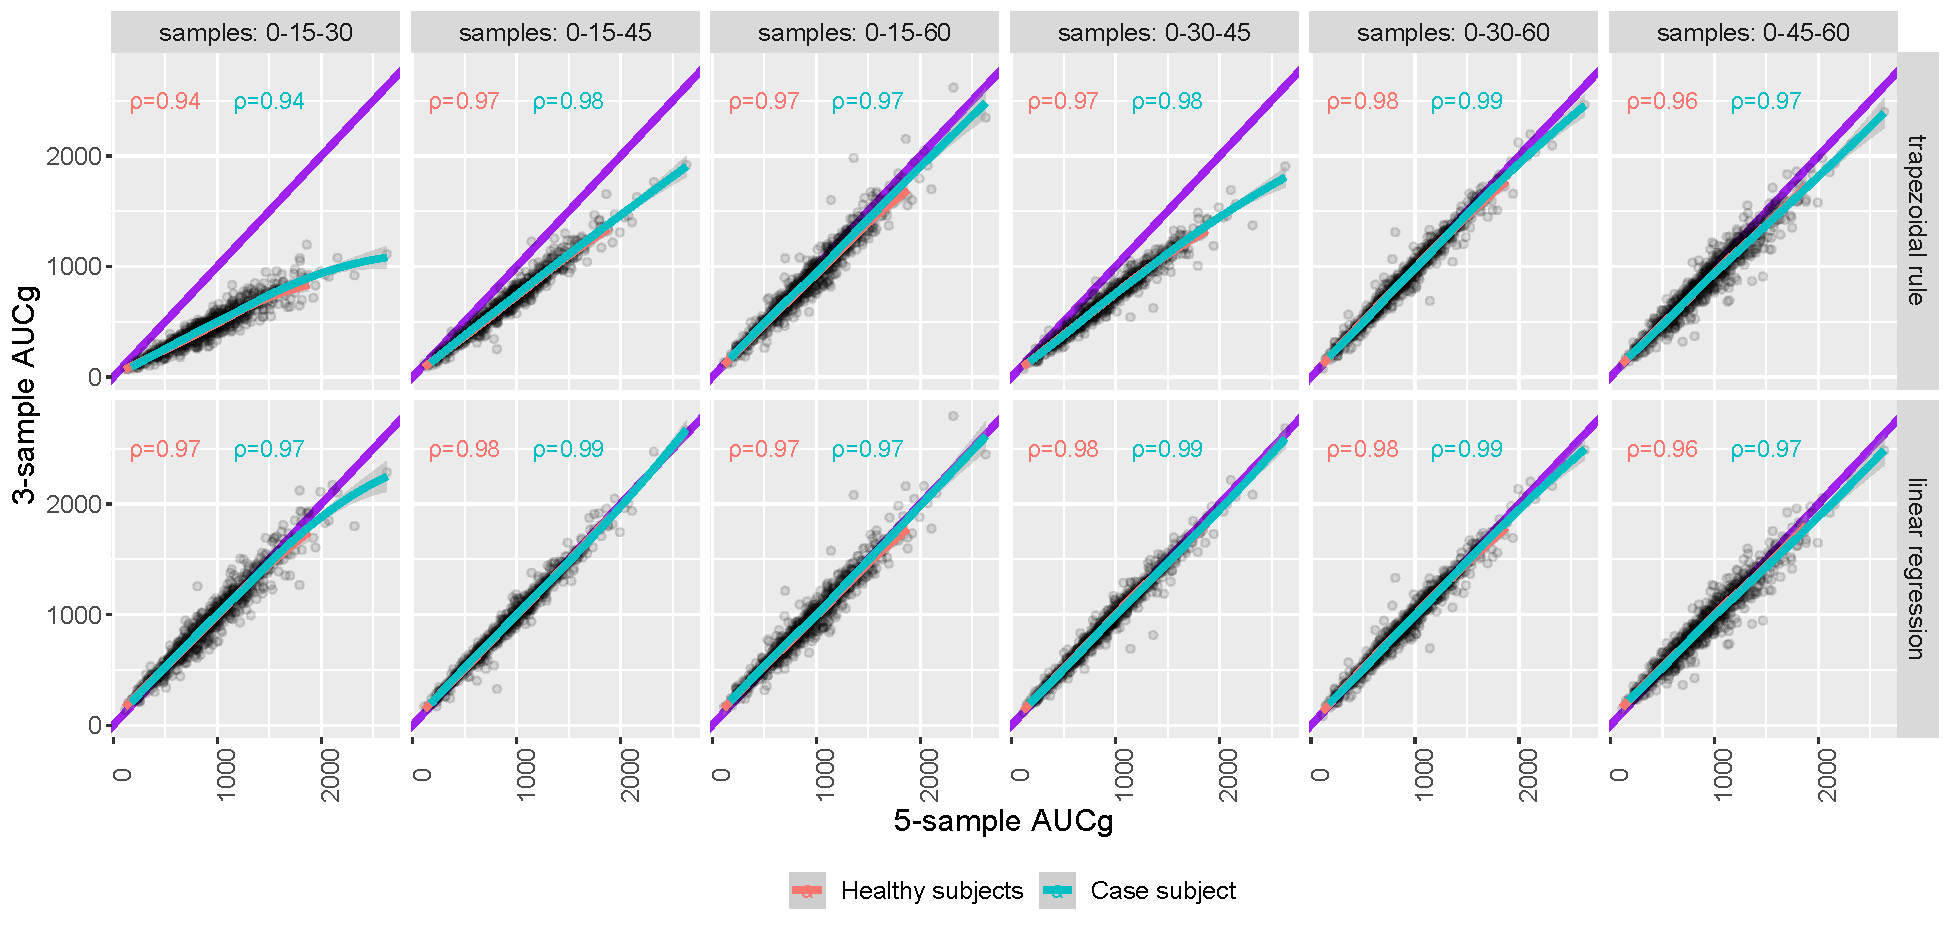
\includegraphics[width=1\textwidth]{./figures/AUCg-perf-cor.pdf}
\caption{\label{fig:AUCg-cor-estimator}Correlation between the estimated 5-sample \(AUC_G\) and the estimated 3-sample \(AUC_G\). The estimates for both the healthy individuals and the patients are displayed (black points). The colored lines show the trend separately for the healthy individuals and the patients (not always visible because they are essential the same). The purple line is the identity line (i.e. no bias).}
\end{figure}

\begin{figure}[!h]
\centering
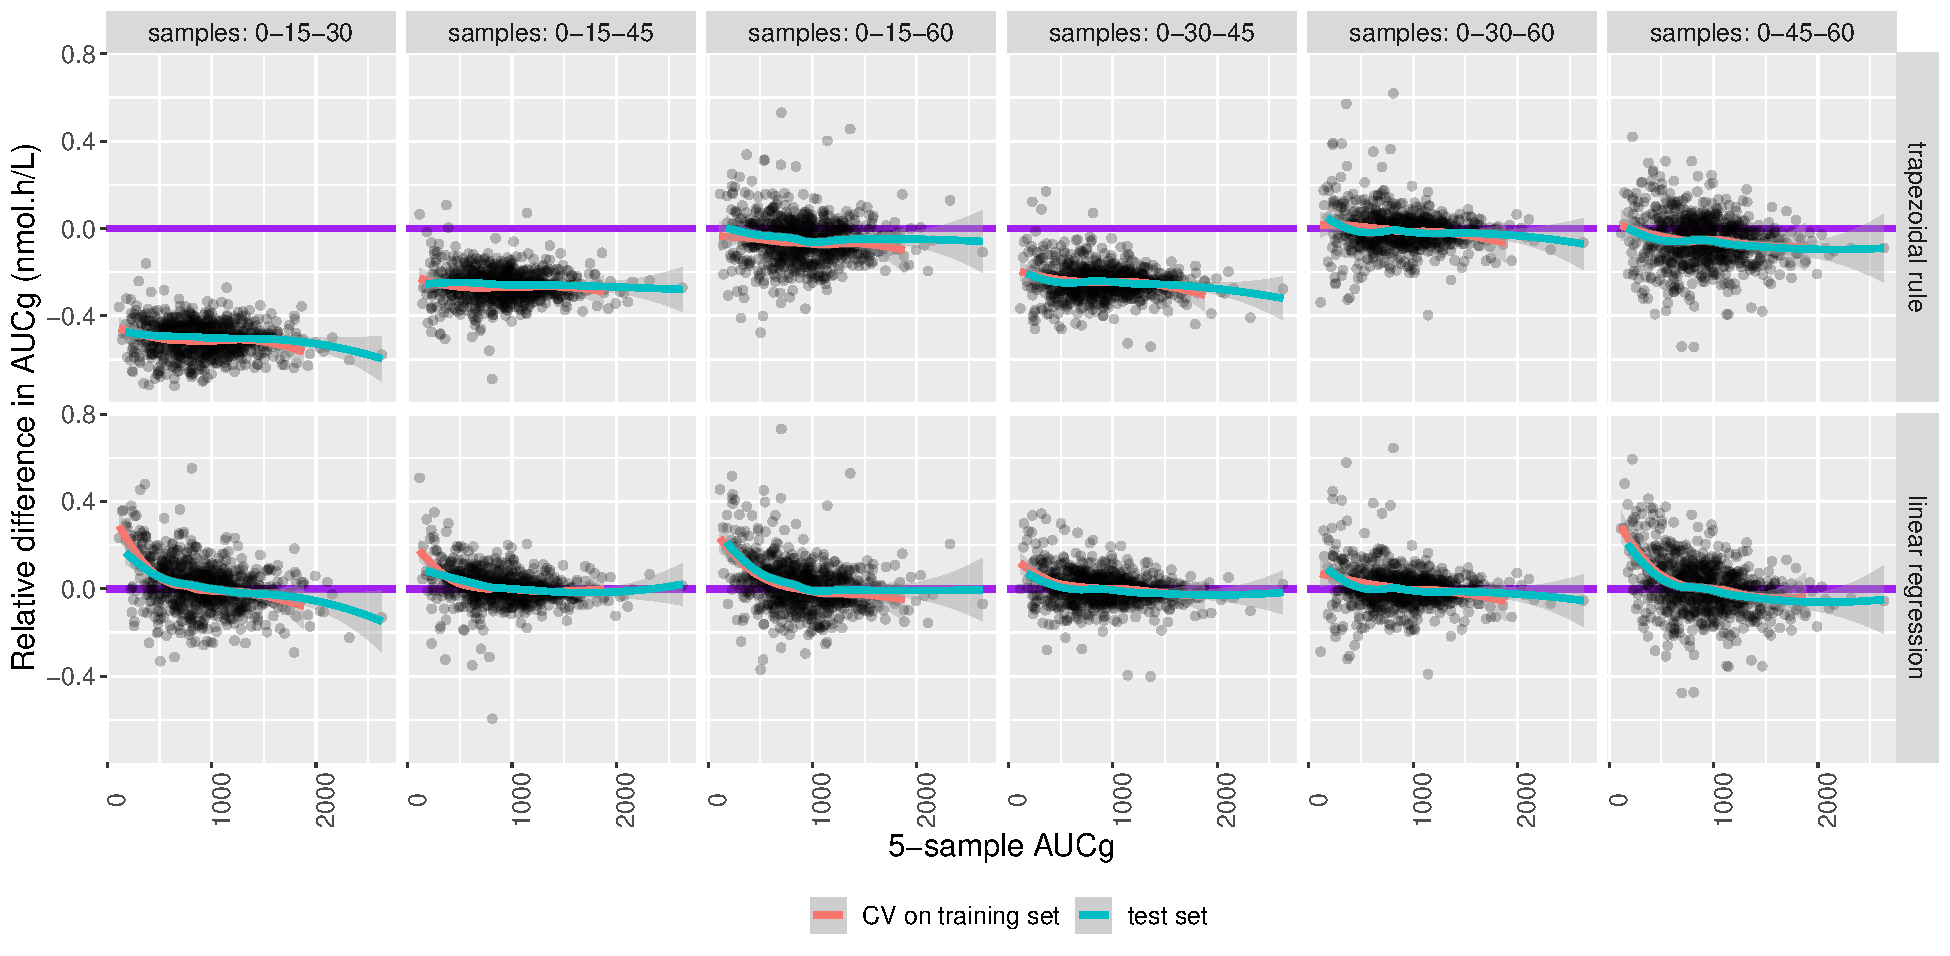
\includegraphics[width=1\textwidth]{./figures/AUCg-perf-blandRelative.pdf}
\caption{\label{fig:AUCg-bland-estimator}Relative error as a function of the estimated 5-sample \(AUC_G\). The estimates for both the healthy individuals and the patients are displayed (black points). The colored lines show the trend separately for the healthy individuals and the patients (not always visible because they are essential the same). The purple line corresponds to no bias.}
\end{figure}

\clearpage

\subsection{Evaluation of the estimators: 3 vs. 5-sample \(AUC_I\)}
\label{sec:orgc27fb62}

Results for the \(AUC_I\) are rather similar to the \(AUC_G\),
e.g. see \autoref{fig:AUCi-perf-estimator},
\autoref{fig:AUCi-cor-estimator} and \autoref{tab:AUCi-perfEstimator}. The
main difference is that the correlation was a bit lower. This can be
easily explained: the error was the same as for the \(AUC_G\), so
since the \(AUC_G\) is larger (in absolute value) compared to the
\(AUC_I\), the variability was higher. 

\begin{figure}[!h]
\centering
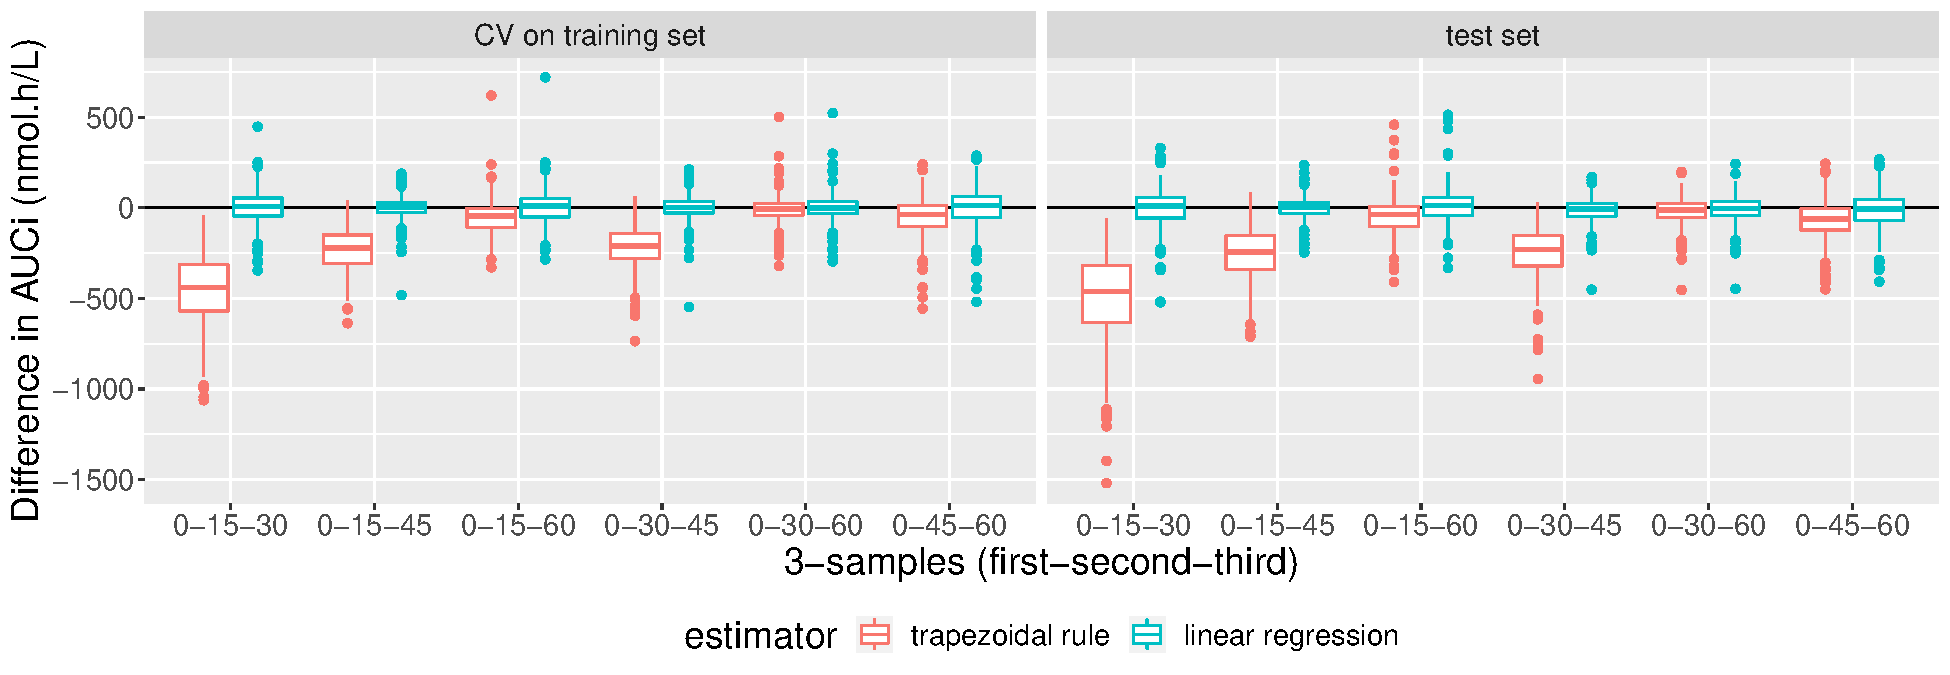
\includegraphics[width=1\textwidth]{./figures/AUCi-perf-boxplot.pdf}
\caption{\label{fig:AUCi-perf-estimator}Boxplot of the difference between the estimated 5-sample \(AUC_I\) and the estimated 3-sample \(AUC_I\). The closer to 0 the better.}
\end{figure}

\begin{figure}[!h]
\centering
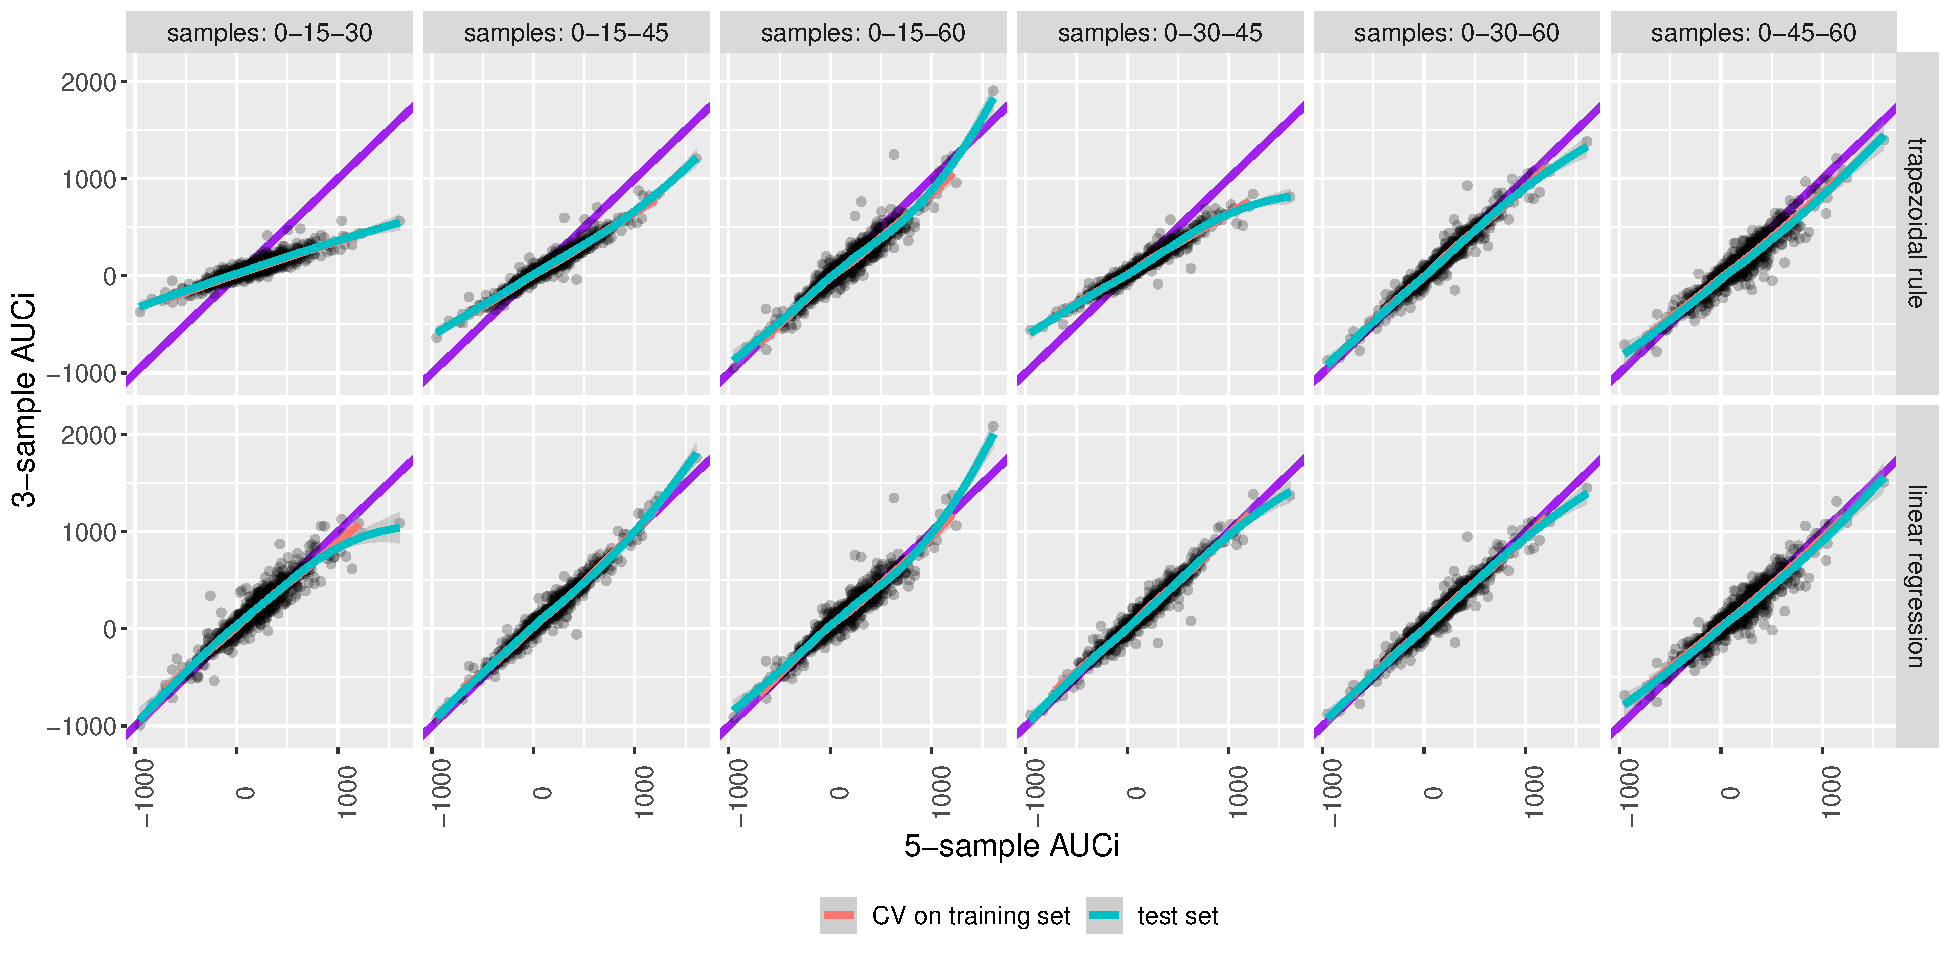
\includegraphics[width=1\textwidth]{./figures/AUCi-perf-cor.pdf}
\caption{\label{fig:AUCi-cor-estimator}Correlation between the estimated 5-sample \(AUC_I\) and the estimated 3-sample \(AUC_I\). The estimates for both the healthy individuals and the patients are displayed (black points). The colored lines show the trend separately for the healthy individuals and the patients (not always visible because they are essential the same). The purple line is the identity line (i.e. no bias).}
\end{figure}

\FloatBarrier
\clearpage

\section{Application of the 3-sample AUC}
\label{sec:orga2f9b4c}
\subsection{Re-analysis of \citep{jakobsen2016brain}}
\label{sec:org6df9709}

We will now replicate the study of Jakobsen et al (2016).

\bigskip

\textbf{Data management}: 1 subject (50678) had missing wake-up time and
another (50524) had missing time for sample. Both were assigned the
most likely time with respect to how the other sample were taken. It
turns out that the other samples were all on schedule (e.g. 15 minutes
between sample 4 and 5) so the assigned values lead to perfect
adherence to planned schedule. See \autoref{fig:jak-descriptive} for a
graphical display of the data.

\begin{figure}[!h]
\centering
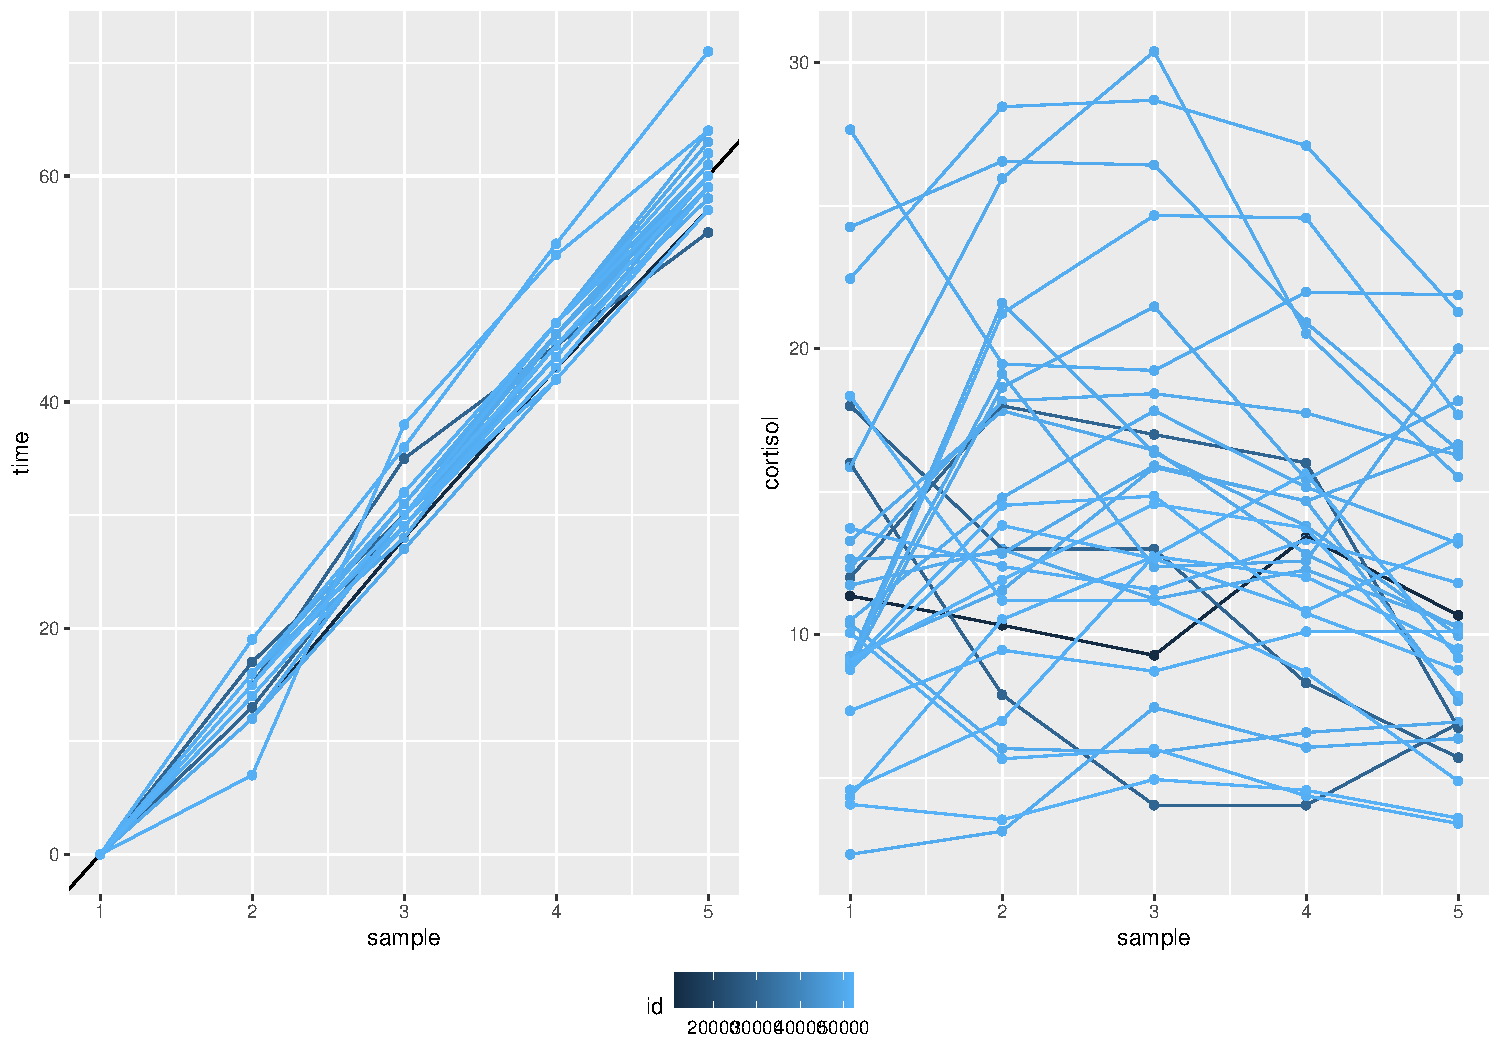
\includegraphics[width=1\textwidth]{./figures/gg-jak-descriptive.pdf}
\caption{\label{fig:jak-descriptive}Left panel: time at which the sample were taken. Right panel: cortisol values per individual.}
\end{figure}


\bigskip

\textbf{AUC calculation (5 samples)}: the AUCg and AUCi computed in R exactly
 matched the one from the database.

\bigskip

\textbf{AUC calculation (3 samples)}: We focused on the 3-sample AUC with the
sample taken at 0, 30, and 60 minutes. The discrepancy with the
5-sample AUC is shown on \autoref{fig:jak-errorAUC}. For the AUCg the
error varied -66.35 to +139.53. Relatively to the 5-sample AUC value,
it varied between -13.61\% and +17.96\%. There was a tendency for a too
low estimated value when using the 3-sample approach (-20.983,
p=0.0339). There was no evidence that the error was AUC dependent for
the AUCg (p=0.276) while there was rather strong evidence in favor of
a linear trend for the AUCi (slope=0.1, p=0.002). 

\begin{figure}[!h]
\centering
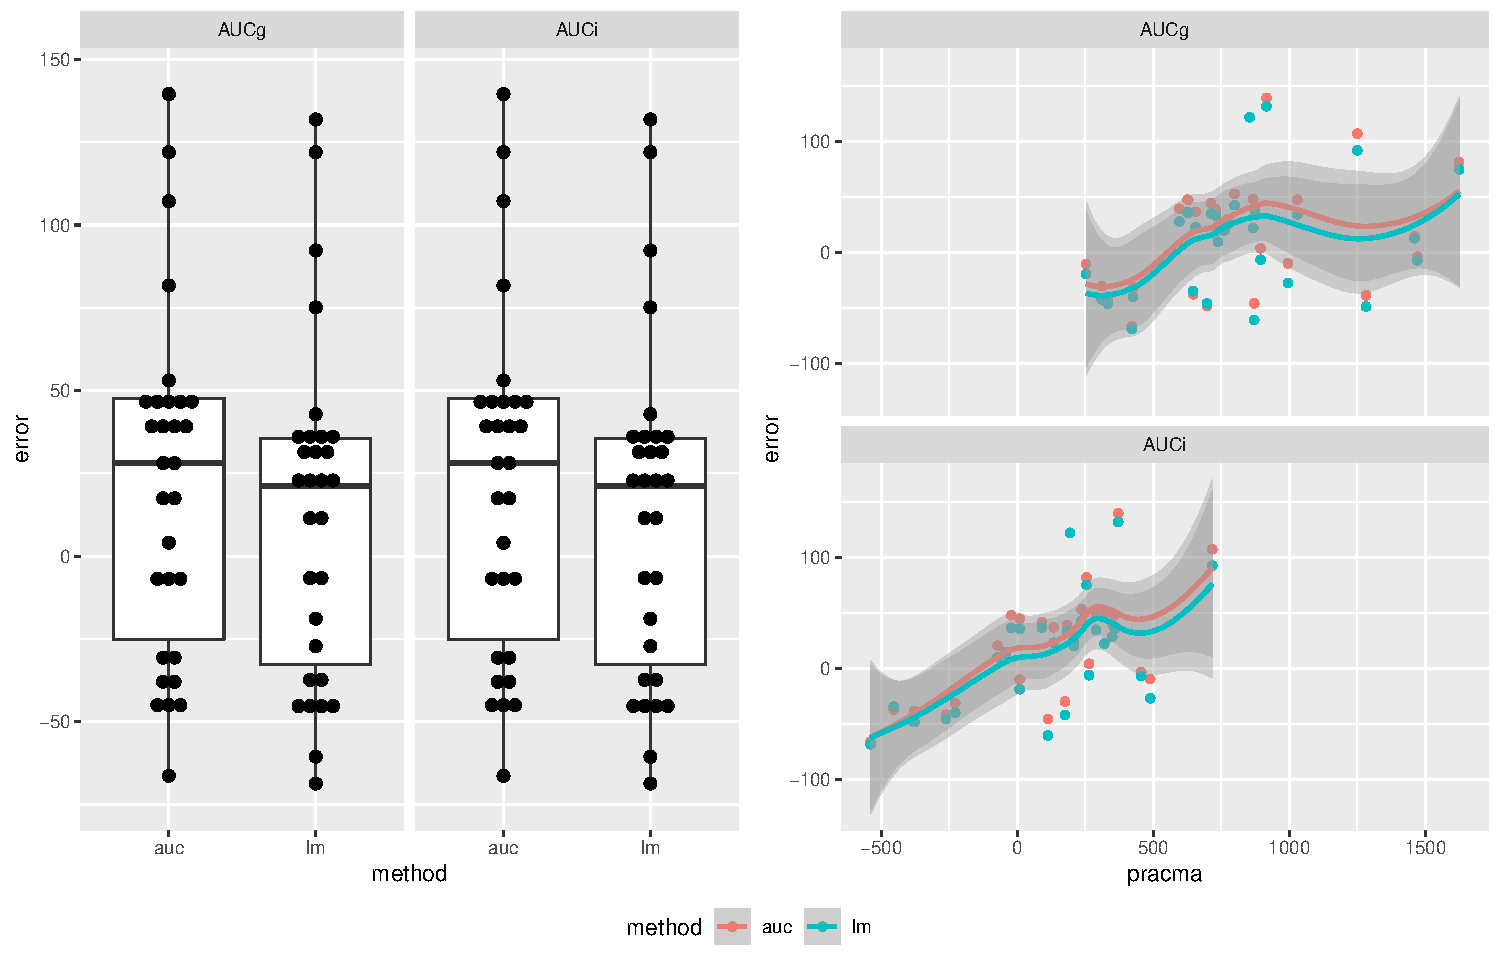
\includegraphics[width=1\textwidth]{./figures/gg-jak-errorAUC.pdf}
\caption{\label{fig:jak-errorAUC}First two panels: boxplot of discrepancy between 3- and 5-sample AUC by estimator. Last two panels: discrepancy between 3- and 5-sample AUC along the 5-sample AUC value.}
\end{figure}

\bigskip

\textbf{Estimation of the association binding-cortisol}: \autoref{tab:Jak2016} shows
the estimated effect when using 3- or 5- samples to compute the
AUC. The effect seems a little bit attenuated and its estimation a bit
less uncertain. Overall the p-values are very similar.

\subsection{Re-analysis of Frokjaer et al 2014}
\label{sec:org9183b88}

We will now replicate the analysis of Frojkaer et al (2014).

\textbf{Data management}: 2 subject had missing cortisol level at one
timepoint. Subject 11083 (Case) was missing the 4th value and subject
11101 was missing the 5th value. See \autoref{fig:fro-descriptive} for a graphical display of the
data:

\begin{figure}[!h]
\centering
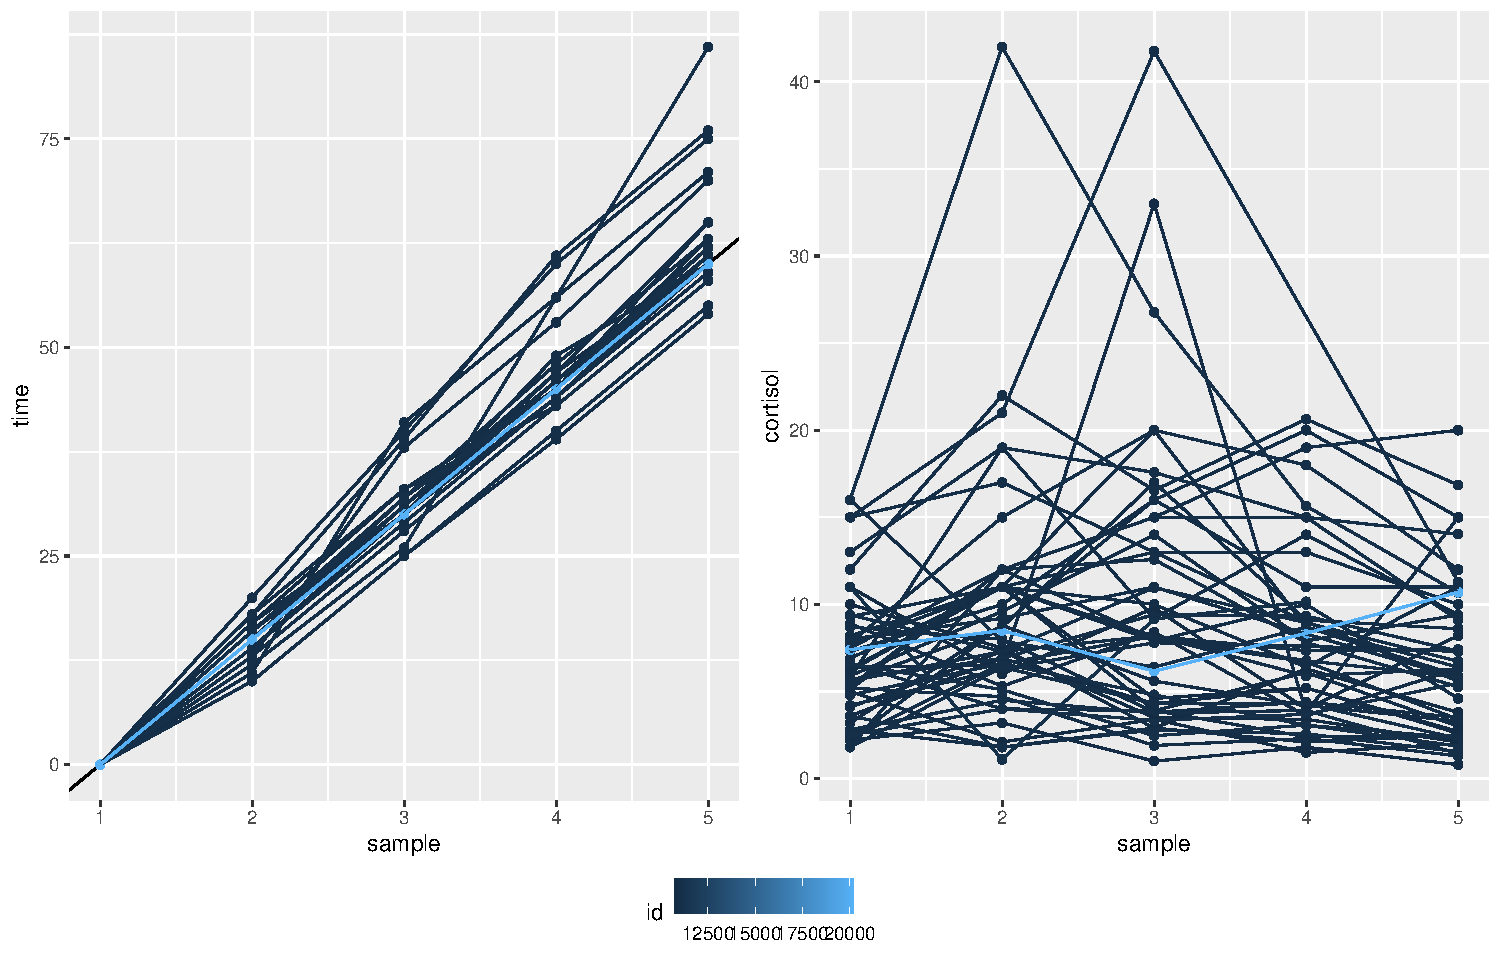
\includegraphics[width=0.9\textwidth]{./figures/gg-fro-descriptive.pdf}
\caption{\label{fig:fro-descriptive}Left panel: time at which the sample were taken. Right panel: cortisol values per individual.}
\end{figure}

\bigskip

\textbf{AUC calculation (5 samples)}: the AUCi computed in R excactly matched
the one from the database.

\bigskip

\textbf{AUC calculation (3 samples)}: We focused on the 3-sample AUC with the
sample taken at 0, 30, and 60 minutes. The \texttt{lm} could not estimate the
AUC for the individual missing the 5th cortisol measurement. The
discrepancy with the 5-sample AUC is shown on
\autoref{fig:fro-errorAUC}. For the AUCg the error varied -501.0 to
+322.4, which relatively to the 5-sample AUC value, corresponds to
-38.21 and +54.97\%. 4 observations were driving the error; for the
rest of the observations the error varied between -141 and +123.75
(-24.32\% and 51.07\%). There was no evidence for a biased estimate when
using the 3-sample approach (e.g. AUCi p=0.304, AUCg p=0.419 with the
trapezoidal rule).

\begin{figure}[!h]
\centering
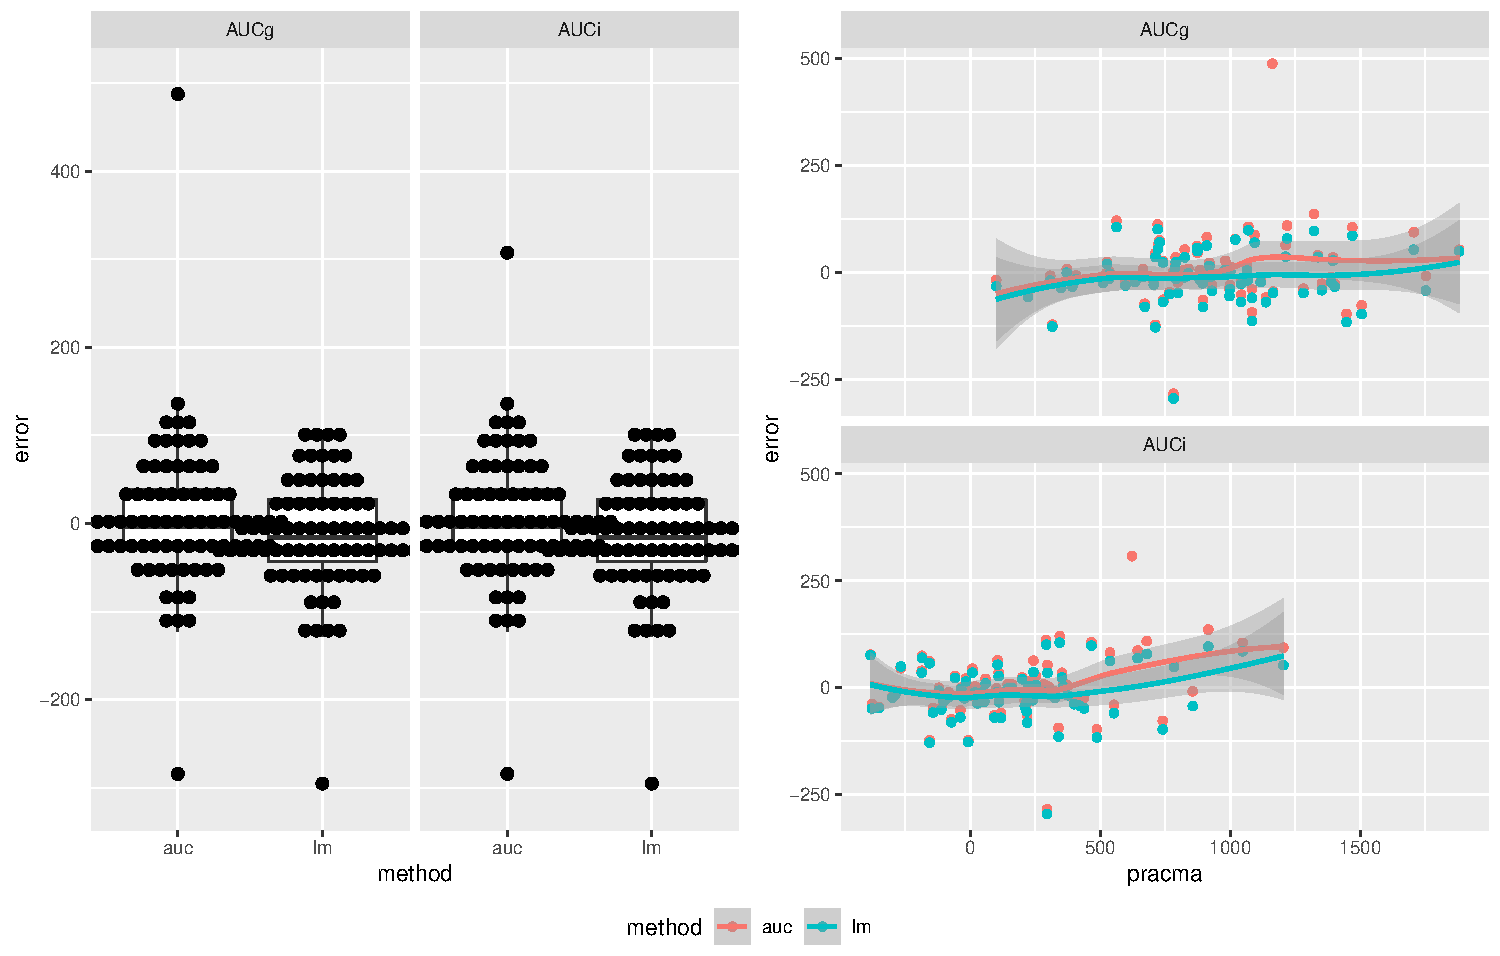
\includegraphics[width=1\textwidth]{./figures/gg-fro-errorAUC.pdf}
\caption{\label{fig:fro-errorAUC}First two panels: boxplot of discrepancy between 3- and 5-sample AUC by estimator. Last two panels: discrepancy between 3- and 5-sample AUC along the 5-sample AUC value.}
\end{figure}

\textbf{Estimation of the association binding-cortisol}: \autoref{tab:Fro2014}
shows the estimated effect when using 3- or 5- samples to compute the
AUC. The effect seems rather similar but with larger standard error
leading to larger p-values.

\clearpage

\section{Conclusion}
\label{sec:org92bc790}

We have shown that the best estimators of the \(AUC_G\) are:
\begin{itemize}
\item the 0-30-60 with the trapezoidal rule
\item the 0-15-45 or 0-30-45 with the linear regression
\end{itemize}
They exhibit a bias close to 0 and a typical fluctuation in \(AUC_G\)
of 60-80 nmol.h/L (about 7-9\%) when compared to the 5-sample
\(AUC_G\). The same error 60-80 nmol.h/L was observed for the
\(AUC_I\) which means that in relative terms (i.e. \%) the 3-samples
was less precise for the \(AUC_I\) than for the \(AUC_G\)\footnote{it is important to keep in mind that an error of 60 may be
small if the true value is 600 but may be large if the true value
is 100.}.

\bigskip

The "best" estimator may also depend on other considerations:
\begin{itemize}
\item which sampling scheme is the most convenient. In particular is it
convenient to avoid the 60 minutes and have instead to do a 45
minutes measurement.
\item whether one is willing to use a data-driven approach (linear
regression) instead of the well established trapezoidal rule.
\end{itemize}

\bigskip

However we must be aware that so far we used the 5-sample \(AUC_G\) as
a reference, which may not give a perfect picture of the true
\(AUC_G\). Therefore we can only claim that (i) the recommanded
3-sample estimators are not more biased than 5-sample estimators and
(ii) derive an upper bound for the loss in precision (here 60-80
nmol.h/L, 7-9\%).  It is also important to realize that these results
may be very specific to the \(AUC\)-statistic. Other summary
statistics, such as peak value may be much more affected by the
reduction of the number of samples.

\bigskip

Finally so far we haven't used any covariate such as age, gender,
\ldots. They could for instance be used to see whether they explain
the heterogeneity in cortisol values or in the shape of the cortisol
trajectory (increasing, decreasing, V-shape).

\clearpage 

\section{Tables}
\label{sec:org503929d}

\begin{table}[!h]
\centering
\begin{tabular}{rrrrrrrr}
  \hline
\multicolumn{8}{l}{Common residual variance-covariance}  \\ 
nb. classes & loglik & cv & nb. parameters & AIC & BIC & SABIC & entropy \\ 
  \hline
1.00 & -6635.30 & 1.00 & 21.00 & 13312.61 & 13399.59 & 13332.94 & 1.00 \\ 
  2.00 & -6586.74 & 1.00 & 27.00 & 13227.47 & 13339.31 & 13253.62 & 0.91 \\ 
  3.00 & -6587.36 & 1.00 & 33.00 & 13240.73 & 13377.42 & 13272.68 & 0.70 \\ 
  4.00 & -6512.69 & 1.00 & 39.00 & 13103.38 & 13264.92 & 13141.14 & 0.88 \\ 
  5.00 & -6515.22 & 1.00 & 45.00 & 13120.43 & 13306.82 & 13164.00 & 0.87 \\ 
  6.00 & -6456.58 & 1.00 & 51.00 & 13015.16 & 13226.40 & 13064.54 & 0.85 \\ 
\hline 
%&&&&&&&&\\
  \hline
\multicolumn{8}{l}{Group specific residual variance-covariance}  \\ 
nb. classes & loglik & cv & nb. parameters & AIC & BIC & SABIC & entropy \\ 
  \hline
1.00 & -6635.30 & 1.00 & 21.00 & 13312.61 & 13399.59 & 13332.94 & 1.00 \\ 
  2.00 & -6505.25 & 1.00 & 28.00 & 13066.50 & 13182.48 & 13093.62 & 0.58 \\ 
  3.00 & -6435.97 & 1.00 & 35.00 & 12941.95 & 13086.92 & 12975.84 & 0.79 \\ 
  4.00 & -6409.37 & 1.00 & 42.00 & 12902.74 & 13076.71 & 12943.41 & 0.79 \\ 
  5.00 & -6389.42 & 1.00 & 49.00 & 12876.84 & 13079.80 & 12924.28 & 0.71 \\ 
  6.00 & -6393.03 & 1.00 & 56.00 & 12898.06 & 13130.01 & 12952.28 & 0.75 \\ 
   \hline
\end{tabular}
\caption{Convergence (column cv, 0 indicates convergence issue) and information criteria for the two LCMM. For AIC, BIC, SABI the lower the better while for entropy the higher the better.}
\label{tab:lcmm}
\end{table}

\begin{table}[ht]
\centering
\begin{tabular}{rllll}
  \hline
Samples & (Intercept) & sample 1 & sample 2 & sample 3 \\ 
  \hline
0-15-30 & 48.96 [26.91;71] & 0.01 [-0.26;0.28] & 0.07 [-0.09;0.23] & 3.14 [2.89;3.38] \\ 
  0-15-45 & 30.43 [15.74;45.12] & 0.04 [-0.13;0.22] & -0.02 [-0.08;0.04] & 0.91 [0.84;0.98] \\ 
  0-15-60 & 41.37 [19.43;63.32] & -0.02 [-0.29;0.24] & -0.08 [-0.14;-0.01] & 0.17 [0.1;0.23] \\ 
  0-30-45 & 18.67 [2.95;34.39] & -0.05 [-0.13;0.03] & 0.07 [0;0.14] & 1.6 [1.4;1.79] \\ 
  0-30-60 & 9.28 [-7.97;26.53] & -0.05 [-0.13;0.04] & -0.02 [-0.07;0.03] & 0.09 [0;0.19] \\ 
  0-45-60 & 42.74 [18.14;67.34] & -0.05 [-0.13;0.03] & 0.02 [-0.07;0.1] & 0.15 [-0.21;0.5] \\ 
   \hline
\end{tabular}
\caption{Coefficients of the linear regression for correcting the trapezoidal rule.}
\label{tab:coeflm}
\end{table}

\clearpage

\begin{table}[ht]
\begin{adjustwidth}{-1cm}{}
\centering
\begin{tabular}{lllllllr}
  \hline
dataset & method &  & median & q. 2.5\% & q. 97.5\% & IQR & cor. \\ 
  \hline
training & auc & 0-15-30 & -440 (-50.5\%) & -847 (-65.7\%) & -114 (-37.2\%) & 256 (10.3\%) & 0.94 \\ 
  (with CV) &  & 0-15-45 & -221 (-26.8\%) & -456 (-39.5\%) & -46 (-13\%) & 156 (8.7\%) & 0.97 \\ 
   &  & 0-15-60 & -45 (-5.8\%) & -241 (-24.7\%) & 92 (15.7\%) & 105 (11.7\%) & 0.97 \\ 
   &  & 0-30-45 & -210 (-24.5\%) & -451 (-38.3\%) & -33 (-8\%) & 138 (7.5\%) & 0.97 \\ 
   &  & 0-30-60 & -8 (-1.1\%) & -139 (-18.1\%) & 107 (17.2\%) & 65 (8.3\%) & 0.98 \\ 
   &  & 0-45-60 & -36 (-4.9\%) & -248 (-28.4\%) & 105 (17.2\%) & 118 (13.4\%) & 0.96 \\ [1mm]
   & lm & 0-15-30 & 8 (1\%) & -199 (-20.1\%) & 173 (25.8\%) & 99 (12.8\%) & 0.97 \\ 
   &  & 0-15-45 & 4 (0.5\%) & -118 (-12\%) & 111 (16.9\%) & 57 (7\%) & 0.98 \\ 
   &  & 0-15-60 & 9 (1\%) & -185 (-17.9\%) & 151 (28.7\%) & 101 (12.7\%) & 0.97 \\ 
   &  & 0-30-45 & 2 (0.2\%) & -119 (-14\%) & 119 (19.5\%) & 64 (8.1\%) & 0.98 \\ 
   &  & 0-30-60 & 0 (0\%) & -131 (-16.9\%) & 122 (18.1\%) & 68 (8\%) & 0.98 \\ 
   &  & 0-45-60 & 14 (1.7\%) & -185 (-20.8\%) & 156 (30.2\%) & 116 (15\%) & 0.96 \\ [3mm]
  test set & auc & 0-15-30 & -463 (-50\%) & -1092 (-65\%) & -119 (-36.9\%) & 314 (10.1\%) & 0.94 \\ 
   &  & 0-15-45 & -244 (-25.8\%) & -536 (-39.4\%) & -55 (-11.7\%) & 186 (8.2\%) & 0.98 \\ 
   &  & 0-15-60 & -38 (-4.3\%) & -248 (-22.7\%) & 107 (14.2\%) & 113 (11.5\%) & 0.97 \\ 
   &  & 0-30-45 & -231 (-25.1\%) & -528 (-38.9\%) & -44 (-10.5\%) & 167 (7.5\%) & 0.98 \\ 
   &  & 0-30-60 & -12 (-1.5\%) & -182 (-18.6\%) & 97 (15.1\%) & 78 (8.3\%) & 0.99 \\ 
   &  & 0-45-60 & -62 (-6.3\%) & -299 (-28.2\%) & 119 (17.2\%) & 118 (11.2\%) & 0.97 \\ 
   & lm & 0-15-30 & 10 (1.3\%) & -232 (-18.8\%) & 143 (21.9\%) & 113 (12.7\%) & 0.97 \\ [1mm]
   &  & 0-15-45 & 3 (0.3\%) & -115 (-11.5\%) & 116 (17.6\%) & 61 (8\%) & 0.99 \\ 
   &  & 0-15-60 & 11 (1.5\%) & -186 (-16.7\%) & 160 (26.6\%) & 101 (11.5\%) & 0.97 \\ 
   &  & 0-30-45 & -8 (-0.7\%) & -149 (-13.4\%) & 103 (12.6\%) & 71 (7.5\%) & 0.99 \\ 
   &  & 0-30-60 & -3 (-0.4\%) & -166 (-17.2\%) & 105 (16.5\%) & 79 (8.6\%) & 0.99 \\ 
   &  & 0-45-60 & -8 (-0.8\%) & -241 (-20.9\%) & 177 (28.8\%) & 116 (12\%) & 0.97 \\ 
   \hline
\end{tabular}
\caption{Discrepancy of the proposed 3-sample estimators with the 5-sample \(AUC_G\) estimated with the trapezoidal rule.
q. 2.5\% and q. 97.5\% stand for 2.5 and 97.5 quantile, IQR for interquartile range, cor. for correlation,
auc for \(AUC_G\) estimated with the trapezoidal rule, lm for \(AUC_G\) estimated using a linear regression.
The column median indicates the median bias (the closer to 0 the higher the accuracy).
The column IQR reflect the precision of the estimator (the lower the better).}
\label{tab:AUCg-perfEstimator}
\end{adjustwidth}
\end{table}

\begin{table}[ht]
\centering
\begin{tabular}{lllrrrrr}
  \hline
dataset & method & timepoint & median & q. 2.5\% & q. 97.5\% & IQR & cor \\ 
  \hline
  \hline
training & auc & 0-15-30 & -85.00 & -448.00 & 272.00 & 212.00 & 0.90 \\ [1mm]
  (with CV) &  & 0-15-45 & -51.00 & -271.00 & 148.00 & 134.00 & 0.96 \\ 
   &  & 0-15-60 & -45.00 & -241.00 & 92.00 & 105.00 & 0.94 \\ 
   &  & 0-30-45 & -37.00 & -265.00 & 194.00 & 114.00 & 0.97 \\ 
   &  & 0-30-60 & -8.00 & -139.00 & 107.00 & 65.00 & 0.97 \\ 
   &  & 0-45-60 & -36.00 & -248.00 & 105.00 & 118.00 & 0.93 \\ 
   & lm & 0-15-30 & 11.00 & -202.00 & 181.00 & 109.00 & 0.94 \\ 
   &  & 0-15-45 & 5.00 & -113.00 & 112.00 & 60.00 & 0.97 \\ 
   &  & 0-15-60 & 9.00 & -185.00 & 151.00 & 101.00 & 0.94 \\ 
   &  & 0-30-45 & 2.00 & -119.00 & 134.00 & 63.00 & 0.97 \\ 
   &  & 0-30-60 & -0.00 & -131.00 & 122.00 & 68.00 & 0.97 \\ 
   &  & 0-45-60 & 14.00 & -185.00 & 156.00 & 116.00 & 0.93 \\  [3mm]
  test set & auc & 0-15-30 & -72.00 & -584.00 & 313.00 & 252.00 & 0.92 \\ 
   &  & 0-15-45 & -43.00 & -340.00 & 214.00 & 158.00 & 0.97 \\ 
   &  & 0-15-60 & -38.00 & -248.00 & 107.00 & 113.00 & 0.96 \\ 
   &  & 0-30-45 & -40.00 & -322.00 & 190.00 & 140.00 & 0.97 \\ 
   &  & 0-30-60 & -12.00 & -182.00 & 97.00 & 78.00 & 0.98 \\ 
   &  & 0-45-60 & -62.00 & -299.00 & 119.00 & 118.00 & 0.95 \\  [1mm]
   & lm & 0-15-30 & 17.00 & -228.00 & 199.00 & 112.00 & 0.94 \\ 
   &  & 0-15-45 & 9.00 & -128.00 & 152.00 & 78.00 & 0.98 \\ 
   &  & 0-15-60 & 11.00 & -186.00 & 160.00 & 101.00 & 0.96 \\ 
   &  & 0-30-45 & 1.00 & -133.00 & 115.00 & 79.00 & 0.98 \\ 
   &  & 0-30-60 & -3.00 & -166.00 & 105.00 & 79.00 & 0.98 \\ 
   &  & 0-45-60 & -8.00 & -241.00 & 177.00 & 116.00 & 0.95 \\ 
   \hline
\end{tabular}
\caption{Discrepancy of the proposed 3-sample estimators with the 5-sample \(AUC_I\) estimated with the trapezoidal rule.
IQR stands for interquartile range, auc for \(AUC_I\) estimated with the trapezoidal rule, lm for \(AUC_I\) estimated using a linear regression.
The column median indicates the median bias (the closer to 0 the higher the accuracy).
The column IQR reflect the precision of the estimator (the lower the better).}
\label{tab:AUCi-perfEstimator}
\end{table}


\begin{table}[!h]
\centering
\begin{tabular}{rrrrrr}
  \hline \multicolumn{6}{c}{Pallidostriatum}  \\
  \\
AUC estimator       & effect   & se      & p-value & lower & upper \\ \hline
AUC with 5 samples & -328.241 & 123.285 & 0.013 & -581.657 & -74.825 \\ 
  AUC with 3 samples & -284.250 & 108.123 & 0.014 & -506.501 & -62.000 \\ 
  LM with 3 samples & -289.480 & 108.821 & 0.013 & -513.165 & -65.795 \\ 
  \hline \\
\hline
\multicolumn{6}{c}{Hippocampus} \\
    \\ 
AUC estimator       & effect   & se      & p-value & lower & upper \\ \hline
AUC with 5 samples & -334.606 & 411.014 & 0.423 & -1179.457 & 510.245 \\ 
  AUC with 3 samples & -315.322 & 358.762 & 0.387 & -1052.767 & 422.124 \\ 
  LM with 3 samples & -334.732 & 361.406 & 0.363 & -1077.612 & 408.149 \\ 
  \hline
\end{tabular}
\caption{Estimate association between the AUCi and the binding potential adjusted for age and gene (LA.LA).}
\label{tab:Jak2016}
\end{table}

\begin{table}[!h]
\centering
\begin{tabular}{rrrrrr}
AUC estimator       & effect   & se      & p-value & lower & upper \\ \hline
AUC with 5 samples & 1715.996 & 594.288 & 0.006 & 519.755 & 2912.237 \\ 
  AUC with 3 samples & 1676.618 & 646.631 & 0.013 & 375.019 & 2978.218 \\ 
  LM with 3 samples & 1716.492 & 656.861 & 0.012 & 393.506 & 3039.478 \\ 
  \hline
\end{tabular}
\caption{Estimate association between the AUCi and DASB adjusted for age and MDMA.}
\label{tab:Fro2014}
\end{table}

\clearpage

\section{References}
\label{sec:orgdb493ee}
\begingroup
\renewcommand{\section}[2]{}
\bibliographystyle{apalike}
\bibliography{bibliography}

\endgroup

\appendix
\titleformat{\section}{\normalfont\Large\bfseries}{Appendix~\thesection}{1em}{}

\clearpage

\section{Appendix: Excluded subjects}
\label{appendix:exclusion}
Id's of the excluded individual
\lstset{language=r,label= ,caption= ,captionpos=b,numbers=none}
\begin{lstlisting}
id.rm
\end{lstlisting}

\begin{verbatim}
$interval.awaket0
 [1] "50473"    "50542"    "52514_I1" "11128"    "50219"    "50583"   
 [7] "50753"    "51738_I2" "51995_I1" "52168_I2" "52463_I3" "52645_I2"
[13] "52687_I1" "52698_I1" "53566"    "55815"   

$interval.t0t15
[1] "52514_I1" "53100_I1" "52184"    "52391_I2" "52594"    "52690_I2" "53809"   
[8] "55059"   

$interval.t15t30
 [1] "52185_I1" "52391_I2" "10909"    "10999"    "11041"    "30048"   
 [7] "30156"    "50127_I1" "50276"    "50682"    "51756_I1" "52115_I1"
[13] "52495_I1" "52594"    "53010_I1" "53350"    "53619"    "53882"   
[19] "53888_I2" "55796_I2"

$interval.t30t45
 [1] "50798_I2" "55264"    "11041"    "11092"    "11140_I3" "30156"   
 [7] "50217"    "50276"    "51411_I1" "51745"    "51918_I2" "52235_I2"
[13] "52470_I2" "52579_I1" "52661_I2" "52687_I2" "53882"    "55777_I1"

$interval.t45t60
 [1] "50752_I2" "53062_I2" "53639"    "10960"    "11083"    "30156"   
 [7] "50276"    "50327"    "50682"    "50705_I1" "51749_I1" "52104_I1"
[13] "52151_I2" "52621"    "52690_I1" "52704_I1" "52711"    "53103_I3"
[19] "53122_I3" "53595"    "53882"    "55121"    "55264"   

$na.cortisol
 [1] "10987"    "11077"    "11080"    "11083"    "11086"    "11092"   
 [7] "11101"    "11104"    "30003"    "30006"    "30054"    "30066"   
[13] "30141"    "50073_I2" "50219"    "50228"    "50288_I2" "50315"   
[19] "50318"    "50330"    "50336"    "50462"    "50489_I1" "50516_I1"
[25] "50670"    "50681_I1" "50769"    "50798_I1" "51745"    "51798_I2"
[31] "51995_I2" "52030_I1" "52085_I2" "52115_I2" "52145_I3" "52151_I2"
[37] "52190_I2" "52412_I3" "52435_I2" "52460"    "52550"    "53103_I3"
[43] "53103_I4" "53127_I3" "53127_I4" "53206"    "53215_I3" "53215_I4"
[49] "53217_I3" "53217_I4" "53259"    "53304"    "53305"    "53336"   
[55] "53443"    "53505"    "53512"    "53532"    "53545"    "53548"   
[61] "53553"    "53569"    "53704"    "53705"    "53716"    "53777"   
[67] "53814"    "53888_I3" "55032"    "55065"    "55072_I2" "55142"   
[73] "55184"    "55738_I2" "55777_I1" "55792_I1" "55811"    "55999_I2"
[79] "56008"    "56046_I1" "56111_I1" "56137_I2" "56216_I1" "56220_I2"
[85] "56233_I2" "56288"   

$na.time
 [1] "50463"    "50465"    "50473"    "50507_I1" "50507_I2" "50514_I3"
 [7] "50743_I2" "50778_I1" "50822_I2" "51745"    "51939_I2" "52046_I2"
[13] "52085_I1" "52085_I2" "52470_I2" "52523"    "52579_I2" "52632_I3"
[19] "53100_I3" "53247"    "56103_I1"
\end{verbatim}

\bigskip

\textbf{Note}: for some patient the value of \(AUC_g\) is missing even though
there are all cortisol measurements, e.g.:
\lstset{language=r,label= ,caption= ,captionpos=b,numbers=none}
\begin{lstlisting}
dtW.fulldata[is.na(AUCg),.(id2,date,time_wake,AUCg)]
dtW.fulldata[is.na(AUCg),.(id2,time_t0,time_t15,time_t30,time_t45,time_t60)]
dtW.fulldata[is.na(AUCg),.(id2,cortisol_t0,cortisol_t15,cortisol_t30,cortisol_t45,cortisol_t60)]
\end{lstlisting}

\begin{verbatim}
        id2       date time_wake AUCg
1:    50058 19/11/2008   9:30:00   NA
2:    50294 20/01/2010   7:15:00   NA
3:    52041 11/01/2012  12:00:00   NA
4: 52690_I3 22/05/2013   6:40:00   NA
5: 53009_I3 20/06/2013   8:00:00   NA
6:    56177 15/11/2018   7:15:00   NA
        id2  time_t0 time_t15 time_t30 time_t45 time_t60
1:    50058  9:45:00 10:05:00 10:22:00 10:38:00 10:55:00
2:    50294  7:30:00  7:45:00  8:00:00  8:15:00  8:30:00
3:    52041 12:15:00 12:30:00 12:45:00 13:00:00 13:15:00
4: 52690_I3  6:52:00  7:08:00  7:23:00  7:38:00  7:55:00
5: 53009_I3  8:15:00  8:30:00  8:45:00  9:00:00  9:15:00
6:    56177  7:30:00  7:45:00  8:00:00  8:15:00  8:30:00
        id2 cortisol_t0 cortisol_t15 cortisol_t30 cortisol_t45 cortisol_t60
1:    50058        4.60         4.80         3.04         3.55         3.11
2:    50294        8.76        18.38        24.92        27.09        18.09
3:    52041       11.08        11.60        11.91        11.75         9.34
4: 52690_I3       17.66        24.80        22.64        21.69        22.79
5: 53009_I3       21.65        12.79        11.78        16.48         9.65
6:    56177        5.55         4.73        17.22        14.64        13.52
\end{verbatim}

\textcolor{red}{Is that voluntary? Can I use the cortisol values?}

\clearpage

\section{Appendix: calculation of the CAR using the trapezoidal rule}
\label{appendix:trapezRule}
\subsection{AUCg}
\label{sec:org4facb2a}

For subjects with regular measurement times, e.g.:
\lstset{language=r,label= ,caption= ,captionpos=b,numbers=none}
\begin{lstlisting}
keep.col <- c("id", 
	      paste0("cortisol_t",c(0,15,30,45,60)),
	      paste0("time_t",c(0,15,30,45,60)),
	      "AUCg")
dtW.fulldata[2, .SD, .SDcols = keep.col]
\end{lstlisting}

\begin{verbatim}
      id cortisol_t0 cortisol_t15 cortisol_t30 cortisol_t45 cortisol_t60
1: 10837         3.2          8.8          5.6          4.2          3.3
   time_t0 time_t15 time_t30 time_t45 time_t60   AUCg
1: 7:10:00  7:25:00  7:40:00  7:55:00  8:10:00 327.75
\end{verbatim}

the \(AUC_g\) can be computed as a weighted average of the cortisol
measurement with weights \(7.5\), \(15\), \(15\), \(15\), \(7.5\):
\lstset{language=r,label= ,caption= ,captionpos=b,numbers=none}
\begin{lstlisting}
3.2 * 7.5 + 8.8 * 15 + 5.6 *15 + 4.2 * 15 + 3.3 * 7.5
\end{lstlisting}

\begin{verbatim}
[1] 327.75
\end{verbatim}


We can check the result using the \texttt{trapz} function from the \emph{pracma} package in R:
\lstset{language=r,label= ,caption= ,captionpos=b,numbers=none}
\begin{lstlisting}
trapz(x = c(0,15,30,45,60), y = c(3.2,8.8,5.6,4.2,3.3))
\end{lstlisting}

\begin{verbatim}
[1] 327.75
\end{verbatim}


For subjects with irregular measurement times, e.g.:
\lstset{language=r,label= ,caption= ,captionpos=b,numbers=none}
\begin{lstlisting}
dtW.fulldata[1, .SD, .SDcols = keep.col]
\end{lstlisting}

\begin{verbatim}
      id cortisol_t0 cortisol_t15 cortisol_t30 cortisol_t45 cortisol_t60
1: 10834         8.9          5.3          8.4          3.6          6.3
   time_t0 time_t15 time_t30 time_t45 time_t60  AUCg
1: 9:16:00  9:30:00  9:45:00 10:00:00 10:15:00 366.4
\end{verbatim}


the weights need to be adapted. The correct weights correspond to half
of the time interval on each side of the measurement:
\lstset{language=r,label= ,caption= ,captionpos=b,numbers=none}
\begin{lstlisting}
8.9 * (14/2) + 5.3 * (14+15)/2 + 8.4 * (15+15)/2 + 3.6 * (15+15)/2 + 6.3 * 15/2
\end{lstlisting}

\begin{verbatim}
[1] 366.4
\end{verbatim}


\lstset{language=r,label= ,caption= ,captionpos=b,numbers=none}
\begin{lstlisting}
trapz(x = c(0,14,29,44,59), y = c(8.9, 5.3, 8.4, 3.6, 6.3))
\end{lstlisting}

\begin{verbatim}
[1] 366.4
\end{verbatim}


Thus over all patients we get the same AUCg as the one of the database
\lstset{language=r,label= ,caption= ,captionpos=b,numbers=none}
\begin{lstlisting}
range(dtLR.HC$AUCg-dtLR.HC$AUCg.pracma, na.rm=TRUE)
\end{lstlisting}

\begin{verbatim}
[1] -1.023182e-12  1.023182e-12
\end{verbatim}

\subsection{AUCb}
\label{sec:orgad30b84}

Consider the individual:
\lstset{language=r,label= ,caption= ,captionpos=b,numbers=none}
\begin{lstlisting}
keep.col <- c("id", "cortisol_t0",
	      paste0("time_t",c(0,15,30,45,60)),
	      "AUCb")
dtW.fulldata[dtW.fulldata$id=="10837", .SD, .SDcols = keep.col]
\end{lstlisting}

\begin{verbatim}
      id cortisol_t0 time_t0 time_t15 time_t30 time_t45 time_t60   AUCb
1: 10837         3.2 7:10:00  7:25:00  7:40:00  7:55:00  8:10:00 135.75
\end{verbatim}


that has had taken cortisol measurements during 1h. His area under the
curve with respect to the baseline should therefore be:
\lstset{language=r,label= ,caption= ,captionpos=b,numbers=none}
\begin{lstlisting}
3.2*60
\end{lstlisting}

\begin{verbatim}
[1] 192
\end{verbatim}


The database value is difference, 135.75 because it is treated as
special case since the CAR measurement are not monotonically
increasing over time. This however somehow does not impact the AUCi:
\lstset{language=r,label= ,caption= ,captionpos=b,numbers=none}
\begin{lstlisting}
range(dtLR.HC$AUCi-dtLR.HC$AUCi.pracma, na.rm=TRUE)
\end{lstlisting}

\begin{verbatim}
[1] -1.023182e-12  1.023182e-12
\end{verbatim}



\clearpage

\section{Appendix: bias-correction using the linear regression}
\label{appendix:lm}
\subsection{Example}
\label{sec:orge276483}
We start with an example. Consider the following individual:
\lstset{language=r,label= ,caption= ,captionpos=b,numbers=none}
\begin{lstlisting}
dtW.HC[id2=="11008"]
\end{lstlisting}

\begin{verbatim}
      id   id2   AUCg AUCg.pracma  c0 c15 c30 c45 c60
1: 11008 11008 141.75      141.75 2.8 1.8 2.9 2.1 2.5
\end{verbatim}


who perfectly followed the measurement schedule. His \(AUC_g\) with
respect to the ground is:
\lstset{language=r,label= ,caption= ,captionpos=b,numbers=none}
\begin{lstlisting}
GS <- 2.8 * 7.5 + 1.8 * 15 + 2.9 * 15 + 2.1 * 15 + 2.5 * 7.5
GS
\end{lstlisting}

\begin{verbatim}
[1] 141.75
\end{verbatim}


But if we would take only the first three samples we would get:
\lstset{language=r,label= ,caption= ,captionpos=b,numbers=none}
\begin{lstlisting}
estimate <- 2.8 * 7.5 + 1.8 * 15 + 2.9 * 7.5
estimate
\end{lstlisting}

\begin{verbatim}
[1] 69.75
\end{verbatim}


which is way too low. Fortunately we can use the correction proposed in \autoref{tab:coeflm}:
\lstset{language=r,label= ,caption= ,captionpos=b,numbers=none}
\begin{lstlisting}
estimate + 48.96 + 0.01 * 2.8 * 7.5 + 0.07 * 1.8 * 15 + 3.14 * 2.9 * 7.5
\end{lstlisting}

\begin{verbatim}
[1] 189.105
\end{verbatim}

While not perfect, the is much closer to the value obtained with 5 samples.

\subsection{Theory}
\label{sec:orge4d8f6a}

Consider:
\begin{itemize}
\item 3 cortisol measurements \(X_1\), \(X_2\), \(X_3\), at time \(0\), \(t_1\), and \(t_2\).
\item the 5-sample \(AUC_G\).
\item weights corresponding to the time intervals, i.e. \(w_1 =
  \frac{t_1}{2}\), \(w_1 = \frac{t_2}{2}\), and \(w_3 =
  \frac{t_2-t_1}{2}\).
\end{itemize}

The \(AUC_G\) can be computed as:
\begin{align*}
\widetilde{AUC}_G = w_1 * X_1 + w_2 * X_2 + w_3 * X_3
\end{align*}
A more flexible approach would be to estimate it as:
\begin{align*}
\widehat{AUC}_G = \alpha + \beta_1 * w_1 * X_1 + \beta_2 * w_2 * X_2 + \beta_3 * w_3 * X_3
\end{align*}
where \(\alpha\), \(\beta_1\), \(\beta_2\), and \(\beta_3\) are
estimated based on the data to minimize the average squared difference
between the 5-sample \(AUC\) and the estimated one. 

\bigskip

For instance imagine that the cortisol value is constant over
time. Then the area below the curve from 0 to 30 is half of the area
below the curve from 0 to 60. Choosing \(\alpha=0\) and
\(\beta_1=\beta_2=\beta_3\) leads to:
\begin{align*}
\widehat{AUC}_G = 2 * \widehat{AUC}_G
\end{align*}
which fixes the problem.
\end{document}